% ============================================================================
% Corpo do relatório (incluído por resultados_preliminares_pgc3.tex)
% ============================================================================
\chapter{Introdução}
\label{cap:intro}

O projeto investiga, sob perspectiva médica e não iridológica, se correlatos
de biomarcadores oculares do diabetes mellitus tipo 2 (DM2) podem ser
extraídos de fotografias convencionais da íris. A iridologia, que atribui a
regiões da íris a condição de órgãos distantes, não se sustenta quando
avaliada sob protocolos controlados \citep*{Simon1979,Ernst2000}. A
literatura médica, por outro lado, descreve dois grupos de achados oculares
associados ao diabetes: alterações da vascularização da íris, observadas por
angiografia por tomografia de coerência óptica do segmento anterior
\citep*{Roberts2017,Zett2018,Zhou2025}, e alterações do diâmetro pupilar e da
espessura da íris, ligadas à neuropatia autonômica
\citep*{Cahill2001,Cui2024,Thakar2025}. O projeto pergunta se correlatos dessas
grandezas sobrevivem numa fotografia RGB, que não tem a resolução nem a
especificidade daquelas modalidades.

\secao{O pipeline de classificação e os realces disponíveis}

O ponto de partida é o pipeline de classificação desenvolvido na Iniciação
Científica (IC), aqui chamado de \emph{pipeline da IC}. Ele recebe uma
fotografia do olho, segmenta a pupila e o limbo, normaliza o anel da íris
pelo modelo \rs{} de \citet{Daugman2004} numa faixa retangular de
$201\times720$ pixels (raio $\times$ ângulo), aplica um pré-processamento
fotométrico, extrai descritores e treina classificadores clássicos com
validação cruzada estratificada. Os descritores disponíveis são o vetor de
pixels da faixa subamostrada, os padrões binários locais (LBP)
\citep*{Ojala2002}, as estatísticas de coocorrência de níveis de cinza (GLCM)
\citep*{Haralick1973} e estatísticas de intensidade; os classificadores são a
regressão logística (RL), a máquina de vetores de suporte (SVM), a floresta
aleatória (RF), o perceptron multicamadas (MLP) e o AdaBoost.

O pré-processamento desse pipeline dispunha apenas de ajustes de brilho, de
contraste e de equalização de histograma. Para evidenciar a vascularização,
foram incorporados a ele três realces consolidados de estruturas finas, todos
aplicados ao canal verde após a equalização adaptativa CLAHE
\citep*{Zuiderveld1994}: o filtro de \ves{} multiescala de
\citet{Frangi1998}, baseado nos autovalores da matriz hessiana; a resposta
máxima de um banco de filtros de Gabor orientados \citep*{Daugman1985,Jain1991};
e a soma das transformações \tht{} e \bh{} morfológicas em três escalas
\citep*{Soille2004}. Uma quarta opção combina os mapas de Frangi e \bh{} com
pesos 0,6 e 0,4. Diferentemente de brilho e contraste, que apenas reescalam
as intensidades de todos os pixels pela mesma função, esses operadores
consideram a vizinhança de cada pixel e respondem à forma das estruturas; a
Figura~\ref{fig:representacoes}, no Capítulo~\ref{cap:resultados}, mostra o
efeito de cada um numa faixa normalizada. O pipeline também ganhou um
validador da geometria pupila--íris, que calcula a razão $\rho$ entre os
raios da pupila e da íris, a espessura relativa $\tau$ do anel e a
excentricidade $\epsilon$ entre os centros.

\secao{Perguntas desta etapa}

Com os realces e o validador implementados, o orientador propôs duas
perguntas, que organizam este relatório:
\begin{alineas}
  \item \textbf{vascularização}: é possível usar as imagens resultantes dos
  filtros diretamente no pipeline da IC, evitando a criação de descritores
  manuais de vascularização? Caso os resultados fossem ruins, seria
  necessário voltar aos descritores manuais;
  \item \textbf{pupila}: para o diâmetro da pupila e a espessura da íris,
  será necessário criar descritores manuais ou o pipeline só precisaria da
  fotografia da íris?
\end{alineas}

\secao{Contribuições}

As contribuições desta etapa são:
\begin{alineas}
  \item a integração dos realces como entrada direta do pipeline da IC, com a
  opção \texttt{--transform} e o teste \texttt{--vascular-test} em
  \arq{main.py}, sem nenhum descritor novo;
  \item uma auditoria reprodutível da base legada, com leitura segura dos
  arquivos, remoção de cópias exatas, reparo da costura angular e detecção
  das faixas espelhadas (Seção~\ref{sec:base});
  \item uma avaliação de 120 configurações com o mesmo protocolo, incluindo
  correção da variância da validação cruzada repetida, ajuste para
  comparações múltiplas, teste de permutação, ablação do pré-processamento,
  controle de atalho por cor, comparação com descritores manuais, fusão,
  robustez fotométrica e replicação num segundo leiaute da base;
  \item duas análises de controle que localizam a origem do sinal, o
  desespelhamento das faixas e o recorte radial entre estroma e bordas, e que
  mostram que o ganho aparente dos realces nesta base não vem da
  vascularização;
  \item uma demonstração formal e experimental de que a normalização \rs{}
  descarta o tamanho da pupila (Proposição~\ref{prop:invariancia}), com a
  consequência prática de que a geometria precisa entrar no classificador
  como um bloco explícito;
  \item um detector de pupila e limbo por raios em estrela, RANSAC e
  refinamento integro-diferencial, que mede $\rho$ automaticamente, e a
  fusão por empilhamento da textura com a geometria, integrada ao pipeline
  pela opção \texttt{--with-geometry};
  \item a reprodutibilidade de todos os números do texto, gerados pelos
  \emph{scripts} de experimentos, testes automatizados para os componentes
  novos e a correção de dois defeitos do pipeline encontrados no caminho: a
  incompatibilidade do AdaBoost com as versões atuais do scikit-learn e a
  leitura repetida das mesmas fotografias em sistemas de arquivos que não
  diferenciam maiúsculas, que criava cópias entre treino e teste.
\end{alineas}

O Capítulo~\ref{cap:questoes} formaliza as questões e as hipóteses; o
Capítulo~\ref{cap:fundamentacao} reúne a fundamentação; o
Capítulo~\ref{cap:metodos} descreve dados, protocolo e experimentos; o
Capítulo~\ref{cap:resultados} apresenta os resultados; o
Capítulo~\ref{cap:discussao} discute as respostas e as limitações; e o
Capítulo~\ref{cap:conclusao} conclui e propõe os próximos passos.

% ============================================================================
\chapter{Questões de pesquisa e hipóteses}
\label{cap:questoes}

\secao{Questões}

\begin{alineas}
  \item \textbf{Q1}: ao substituir a imagem de entrada do pipeline da IC pela
  imagem realçada, mantidos os descritores, os classificadores e o
  protocolo, o desempenho muda? A mudança depende do conjunto de
  descritores? O ganho, se houver, vem do filtro ou do pré-processamento que
  os filtros compartilham (canal verde com CLAHE)? Ele supera o acaso, resiste
  a perturbações fotométricas e se repete noutra amostra da base?
  \item \textbf{Q2}: a geometria pupila--íris chega ao classificador quando o
  pipeline recebe a fotografia? Se não chega, o que é preciso: descritores
  manuais, a fotografia completa ou ambos? A geometria pode ser medida
  automaticamente com precisão suficiente?
\end{alineas}

\secao{Hipóteses}

\begin{hipotese}[realce como entrada]\label{hip:realce}
O vetor de pixels de uma faixa original é dominado por variações de baixa
frequência, como a iluminação, as sombras das pálpebras e o gradiente radial
do estroma. Os realces removem esse fundo e preservam as estruturas finas.
Espera-se, portanto, que a imagem realçada melhore os classificadores que
recebem os pixels, e que o ganho desapareça quando a entrada passa apenas pelo
pré-processamento comum, sem o filtro. Para descritores de textura calculados
sobre a imagem original, que já resumem a distribuição de intensidades, não
se espera ganho.
\end{hipotese}

\begin{hipotese}[geometria explícita]\label{hip:geometria}
A normalização \rs{} leva o anel da íris a uma faixa de tamanho fixo
independentemente do raio da pupila. Espera-se que a faixa seja
aproximadamente invariante a $\rho$ e que um efeito puramente geométrico seja
invisível para o pipeline que só recebe a faixa, mas recuperável quando
$\rho$, medido na fotografia, entra como descritor explícito.
\end{hipotese}

% ============================================================================
\chapter{Fundamentação teórica}
\label{cap:fundamentacao}

\secao{O pipeline da IC}

A Figura~\ref{fig:pipeline} resume o pipeline e as duas modificações
avaliadas. Na entrada, a segmentação estima os círculos da pupila e do limbo.
A normalização produz a faixa $N(s,\theta)$, com $s\in[0,1]$ da borda pupilar
($s=0$) ao limbo ($s=1$) e $\theta\in[0,2\pi)$. O pré-processamento escolhe um
canal de cor e aplica uma transformação fotométrica; nesta etapa, os realces
de vascularização passam a ser transformações como as demais. Os descritores
podem ser o vetor de pixels da faixa subamostrada por um fator 4
($50\times180=9000$ valores), a textura (histograma de LBP uniforme com 16
vizinhos e raio 2, seis propriedades de GLCM em três distâncias e quatro
direções, e 36 estatísticas de intensidade, num total de 126 valores) ou a
concatenação dos dois, que é o conjunto padrão da IC. Os classificadores
recebem os descritores padronizados (média zero e variância unitária,
estimadas apenas no treino de cada \emph{fold}).

\begin{figure}[htb]
  \centering
  \caption{Pipeline da IC e as duas modificações avaliadas}
  \label{fig:pipeline}
  \begin{tikzpicture}[
      font=\footnotesize, node distance=4mm and 5mm,
      box/.style={draw, rounded corners=2pt, align=center, minimum height=9mm,
                  text width=19mm, fill=white},
      new/.style={box, draw=blue!60!black, fill=blue!6, thick},
      arr/.style={-{Stealth[length=2mm]}, thick}]
    \node[box] (foto) {Fotografia\\do olho};
    \node[box, right=of foto] (seg) {Segmentação\\(pupila e limbo)};
    \node[box, right=of seg] (norm) {Normalização\\\emph{rubber sheet}};
    \node[new, right=of norm] (real) {Realce\\(Frangi, Gabor,\\\emph{black-hat})};
    \node[box, right=of real] (desc) {Descritores\\(pixels, textura)};
    \node[box, below=9mm of desc] (clf) {Classificador\\(RL, SVM, RF,\\MLP, AdaBoost)};
    \node[new, below=9mm of seg] (geo) {Geometria\\$\rho$, $\tau$, $\epsilon$};
    \node[new, left=of clf] (fus) {Fusão por\\empilhamento};
    \draw[arr] (foto) -- (seg);
    \draw[arr] (seg) -- (norm);
    \draw[arr] (norm) -- (real);
    \draw[arr] (real) -- (desc);
    \draw[arr] (desc) -- (clf);
    \draw[arr, blue!60!black] (seg) -- (geo);
    \draw[arr, blue!60!black] (geo) -- (fus);
    \draw[arr, blue!60!black] (fus) -- (clf);
    \node[font=\scriptsize, text=blue!60!black, align=center, above=1mm of real]
      {Q1: imagem filtrada\\como entrada};
    \node[font=\scriptsize, text=blue!60!black, align=left, below=1mm of geo]
      {Q2: a faixa descarta $\rho$; a geometria\\precisa de um caminho próprio};
  \end{tikzpicture}
  \par\medskip
  \footnotesize Fonte: elaborado pelo autor. Em azul, os componentes
  acrescentados nesta etapa.
\end{figure}

\secao{Realces de estruturas finas}

O filtro de \citet{Frangi1998} calcula, em cada escala $\sigma$, os
autovalores $|\lambda_1|\le|\lambda_2|$ da matriz hessiana da imagem suavizada
e atribui a cada pixel a resposta
\begin{equation}
  V_\sigma = \exp\!\left(-\frac{R_B^2}{2\beta^2}\right)
  \left[1-\exp\!\left(-\frac{S^2}{2c^2}\right)\right],
  \qquad R_B=\frac{\lambda_1}{\lambda_2},\quad S=\sqrt{\lambda_1^2+\lambda_2^2},
\end{equation}
nula quando o sinal de $\lambda_2$ não corresponde à polaridade procurada. A
resposta final é o máximo sobre as escalas $\sigma\in\{1,2,3,4\}$, com
$\beta=0{,}5$ e $c=15$. Ela é alta em estruturas alongadas, cuja curvatura é
forte numa direção e fraca na outra, e baixa em regiões homogêneas e em
manchas isotrópicas. O banco de Gabor usa oito orientações, núcleo de
$21\times21$ pixels, $\sigma=4$, comprimento de onda 10 e razão de aspecto
0,5; a resposta é o máximo do valor absoluto entre as orientações. A
morfologia soma as transformações \tht{} (estruturas claras menores que o
elemento estruturante) e \bh{} (estruturas escuras) com elementos
elípticos de 5, 11 e 21 pixels. Os três realces descartam, por construção,
o nível médio e as variações lentas de intensidade.

\secao{Normalização de Daugman e o tamanho da pupila}
\label{sec:invariancia}

Sejam $\mathbf{p}(\theta)=\mathbf{c}_p+r_p\,\mathbf{u}(\theta)$ e
$\mathbf{i}(\theta)=\mathbf{c}_i+r_i\,\mathbf{u}(\theta)$ os pontos dos
círculos da pupila e do limbo na direção
$\mathbf{u}(\theta)=(\cos\theta,-\sin\theta)$. A normalização de
\citet{Daugman2004} define
\begin{equation}
  N(s,\theta)=I\big((1-s)\,\mathbf{p}(\theta)+s\,\mathbf{i}(\theta)\big),
  \qquad s\in[0,1],\ \theta\in[0,2\pi).
  \label{eq:rubber}
\end{equation}
O modelo supõe que o tecido da íris se estica linearmente entre a pupila e o
limbo: um ponto do estroma que ocupa a posição relativa $s$ continua em $s$
quando a pupila muda de tamanho. É por isso que a normalização compensa a
dilatação no reconhecimento de íris.

\begin{proposicao}\label{prop:invariancia}
Se o estroma se deforma segundo o modelo linear de Daugman e o limbo
permanece fixo, a faixa $N$ não depende de $r_p$. Em consequência, nenhum
descritor calculado apenas sobre $N$, e nenhum classificador que receba
apenas esses descritores, pode distinguir duas fotografias que diferem só no
tamanho da pupila.
\end{proposicao}

\begin{proof}
Sejam $I_0$ e $I_1$ fotografias do mesmo olho com raios pupilares $r_0$ e
$r_1$ e o mesmo limbo. Pelo modelo, o ponto de tecido de coordenadas
$(s,\theta)$ aparece em $I_0$ na posição
$(1-s)\,\mathbf{p}_0(\theta)+s\,\mathbf{i}(\theta)$ e em $I_1$ na posição
$(1-s)\,\mathbf{p}_1(\theta)+s\,\mathbf{i}(\theta)$, com a mesma intensidade.
Aplicando a Equação~\eqref{eq:rubber} com os círculos de cada fotografia,
obtém-se $N_0(s,\theta)=N_1(s,\theta)$ para todo $(s,\theta)$. Qualquer função
de $N$ assume, portanto, o mesmo valor nas duas fotografias.
\end{proof}

\begin{corolario}\label{cor:explicito}
Para que o tamanho da pupila influencie a decisão, $\rho=r_p/r_i$ precisa ser
medido na segmentação, antes da normalização, e entregue ao classificador
como descritor explícito.
\end{corolario}

A deformação real do estroma não é exatamente linear
\citep*{Wyatt2000,TomeoReyes2015}, e a dilatação degrada o reconhecimento de
íris justamente porque deixa um traço residual na faixa
\citep*{Hollingsworth2009}. Esse traço é indireto e mistura o tamanho da
pupila com a textura de cada pessoa; a proposição continua indicando que a
faixa não é o meio adequado para transportar $\rho$. Na amostragem, a faixa
também perde resolução radial quando o anel fica mais fino, o que muda a
nitidez sem codificar $\rho$ de forma direta.

Para simular dilatações com o mesmo modelo, é preciso inverter a
Equação~\eqref{eq:rubber}. Para $s$ fixo, os pontos
$(1-s)\,\mathbf{p}(\theta)+s\,\mathbf{i}(\theta)$ formam um círculo de
centro $\mathbf{c}_p+s(\mathbf{c}_i-\mathbf{c}_p)$ e raio $r_p+s(r_i-r_p)$.
Dado um pixel $\mathbf{x}$, com $\mathbf{d}=\mathbf{x}-\mathbf{c}_p$,
$\mathbf{v}=\mathbf{c}_i-\mathbf{c}_p$, $a=r_p$ e $b=r_i-r_p$, a coordenada
$s$ é a raiz de
\begin{equation}
  \big(\lVert\mathbf{v}\rVert^2-b^2\big)s^2
  -2\big(\mathbf{d}\cdot\mathbf{v}+ab\big)s
  +\big(\lVert\mathbf{d}\rVert^2-a^2\big)=0,
  \label{eq:inversa}
\end{equation}
e $\theta$ é o ângulo de $\mathbf{x}$ em relação ao centro do círculo
correspondente. Essa inversa exata permite gerar a mesma fotografia com
outro tamanho de pupila e verificar a Proposição~\ref{prop:invariancia} sem
aproximação geométrica.

\secao{Geometria pupilar: o que a fotografia mede}
\label{sec:geometria}

Numa fotografia frontal, a segmentação fornece $r_p$, $r_i$ e os centros. Daí
saem a razão $\rho=r_p/r_i$, a espessura relativa do anel
$\tau=(r_i-r_p)/r_i$ e a excentricidade
$\epsilon=\lVert\mathbf{c}_p-\mathbf{c}_i\rVert/r_i$. Como $\tau=1-\rho$, o
diâmetro relativo da pupila e a espessura relativa do anel são a mesma
informação. Os diâmetros em pixels dependem da distância e da óptica da
câmera e só se convertem em milímetros com calibração. Uma aproximação usual
toma o diâmetro horizontal visível da íris como régua, com média de
11,7\,mm em adultos \citep*{Rufer2005}; o diâmetro pupilar em milímetros fica
então próximo de $\rho\times 11{,}7$\,mm, com incerteza de alguns por cento
herdada da variação entre pessoas. A espessura anatômica do estroma, por sua
vez, não é visível numa fotografia frontal e exige AS-OCT ou biomicroscopia
ultrassônica \citep*{Cui2024}. O diâmetro pupilar também varia com a
iluminação, a idade e a acomodação \citep*{WatsonYellott2012}; nos estudos
clínicos, a redução associada ao diabetes aparece na pupila adaptada ao
escuro \citep*{Cahill2001}. Uma medida útil de $\rho$ requer, portanto,
iluminação controlada e registrada na aquisição.

\secao{Avaliação estatística}
\label{sec:estatistica}

\textbf{Métricas.} A acurácia balanceada (AB), média da sensibilidade e da
especificidade, não favorece a classe majoritária. A área sob a curva ROC
(AUC) mede a separação dos escores independentemente do limiar
\citep*{HanleyMcNeil1982,Fawcett2006}.

\textbf{Validação cruzada repetida.} Em $r$ repetições de $K$
\emph{folds}, obtêm-se $k=rK$ estimativas que não são independentes, porque
os conjuntos de treino se sobrepõem. O intervalo de confiança da média e o
teste t pareado entre duas configurações usam então a variância corrigida de
\citet{NadeauBengio2003},
\begin{equation}
  \hat\sigma^2_{\text{corr}}=\left(\frac{1}{k}+\frac{n_2}{n_1}\right)\hat\sigma^2,
\end{equation}
em que $\hat\sigma^2$ é a variância amostral das $k$ estimativas (ou das
diferenças) e $n_1$ e $n_2$ são os tamanhos de treino e de teste. A correção
evita a taxa excessiva de falsos positivos do teste t comum
\citep*{BouckaertFrank2004}.

\textbf{Comparações múltiplas.} Famílias de testes recebem o ajuste de
\citet{Holm1979}. Para ordenar várias configurações sobre vários blocos, usa-se
o teste de \citet{Friedman1937}, com a estatística $F$ de
\citet{ImanDavenport1980} e a diferença crítica de \citet{Nemenyi1963},
conforme \citet{Demsar2006}.

\textbf{Teste de permutação.} Para verificar se uma configuração supera o
acaso, os rótulos são permutados e a validação cruzada é refeita
\citep*{OjalaGarriga2010}; o valor $p$ é $(1+b)/(1+B)$, em que $b$ é o número
de permutações com desempenho maior ou igual ao observado entre $B$
permutações \citep*{PhipsonSmyth2010}.

\textbf{Mapas por pixel.} A diferença entre classes em cada pixel da faixa é
medida pelo $d$ de \citet{Cohen1988}, com o teste t de Welch e controle da
taxa de falsas descobertas pelo procedimento de
\citet{BenjaminiHochberg1995}.

% ============================================================================
\chapter{Materiais e métodos}
\label{cap:metodos}

\secao{Base de dados e auditoria}
\label{sec:base}

A única base rotulada disponível é um arquivo legado de faixas já
normalizadas ($201\times720\times3$, BGR), distribuído junto de um artigo
sobre a predição de diabetes por regiões da íris que foi retratado pelo IEEE
\citep*{Moradi2018}. O arquivo traz cinco leiautes (\texttt{all},
\texttt{L\_split}, \texttt{R\_split}, \texttt{personBase} e
\texttt{personBase\_invert}), sem as fotografias originais, sem os contornos,
sem identificadores de pessoa e com a classe positiva definida apenas como
diabetes informado. Por isso a base não permite conclusões clínicas e não é
redistribuída; nenhuma figura deste relatório mostra imagens dela.

A leitura usa um desserializador restrito, que aceita apenas os construtores
do NumPy necessários para reconstruir os arrays e bloqueia qualquer outro
objeto do arquivo. A auditoria (Tabela~\ref{tab:auditoria}) encontrou:
\begin{alineas}
  \item \val{aud-copias} cópias exatas entre as \val{aud-linhas} linhas de
  cada leiaute por pessoa, com uma mesma imagem repetida até
  \val{aud-multmax} vezes. Mantidas, essas cópias cairiam em \emph{folds}
  diferentes e inflariam as métricas; elas foram removidas por SHA-256,
  restando \val{aud-unicas} imagens únicas (\val{aud-controle} controles e
  \val{aud-diabetes} com diabetes informado em \texttt{personBase\_invert});
  \item no leiaute \texttt{personBase\_invert}, as faixas do olho direito
  foram espelhadas: a inversão angular seguida de um deslocamento de 360
  colunas leva o ângulo $\theta$ a $180^\circ-\theta$, isto é, troca os lados
  nasal e temporal, provavelmente para alinhar a anatomia dos dois olhos.
  Desfeita essa transformação, \val{aud-lado-espelhadas-em-R} das
  \val{aud-esp-total} faixas espelhadas coincidem exatamente com faixas do
  leiaute \texttt{R\_split} (olho direito), e \val{aud-lado-nao-espelhadas-em-L}
  das \val{aud-naoesp-total} demais, com faixas do \texttt{L\_split}. A
  costura angular vazia, uma coluna inteiramente nula, aparece na coluna 360
  das faixas espelhadas e na coluna 719 das demais; como ela marca o lado do
  olho, e o lado não está equilibrado entre as classes (\val{aud-esp-controle}
  controles e \val{aud-esp-diabetes} casos espelhados), a coluna foi
  preenchida com a média das vizinhas;
  \item nenhum par de imagens únicas com correlação igual ou superior a 0,97
  (mediana das correlações entre pares: \val{aud-corr-mediana}; máximo:
  \val{aud-corr-max}). Sem identificadores, cada imagem única forma um grupo
  próprio na validação cruzada, e olhos da mesma pessoa podem ficar em
  \emph{folds} diferentes;
  \item uma diferença de cor média entre as classes: o canal azul vale
  \val{aud-b-controle} nos controles e \val{aud-b-diabetes} nos casos, e o
  vermelho, \val{aud-r-controle} e \val{aud-r-diabetes}, enquanto o cinza
  quase não muda. A Seção~\ref{sec:controles} testa se essa diferença basta
  para classificar.
\end{alineas}

\begin{table}[htb]
  \centering
  \caption{Auditoria dos dois leiautes por pessoa da base legada}
  \label{tab:auditoria}
  \footnotesize
  % Gerado por experiments/pgc3_vascular_pipeline.py (não editar à mão).
\begin{tabular}{lcc}
\toprule
Item & \texttt{personBase\_invert} & \texttt{personBase} \\
\midrule
Linhas (controle / diabetes) & 108 / 88 & 108 / 88 \\
Cópias exatas removidas & 73 & 73 \\
Imagens únicas (controle / diabetes) & 66 / 57 & 63 / 60 \\
Maior multiplicidade de uma cópia & 6 & 7 \\
Faixas espelhadas (controle / diabetes) & 30 / 33 & 0 / 0 \\
Coluna nula da costura (coluna: imagens) & 360: 63, 719: 60 & 719: 123 \\
Pares com correlação $\geq 0{,}97$ & 0 & 0 \\
Grupos da validação cruzada & 123 & 123 \\
\bottomrule
\end{tabular}

  \par\medskip
  \footnotesize Fonte: elaborada pelo autor.
\end{table}

O leiaute principal é \texttt{personBase\_invert}, o padrão do código que
acompanha a base legada. O leiaute \texttt{personBase}, que tem o
mesmo número de imagens únicas mas compartilha apenas
\val{aud-compartilhadas} delas com o principal, serve de replicação.

\secao{Representações de entrada}

O Quadro~\ref{qua:representacoes} lista as oito representações. As três
primeiras são as linhas de base do pipeline; a quarta é uma ablação que
aplica o pré-processamento comum dos filtros (canal verde e CLAHE) sem
filtro algum, o que permite atribuir ao filtro, e não ao pré-processamento,
qualquer diferença observada. Os realces usam exatamente os parâmetros
descritos na fundamentação, sem ajuste nos dados desta etapa.

\begin{quadro}[htb]
  \caption{Representações de entrada avaliadas no pipeline da IC}
  \label{qua:representacoes}
  \footnotesize
  \begin{tabular}{p{3.6cm}p{1.6cm}p{8.6cm}}
    \toprule
    Representação & Canal & Operação sobre a faixa \\
    \midrule
    Original & cinza & nenhuma (entrada original do pipeline) \\
    Equalização global & cinza & equalização de histograma global \\
    CLAHE & cinza & equalização adaptativa com limite de contraste 2,0 \\
    Verde + CLAHE & verde & ablação: pré-processamento comum dos filtros,
      sem filtro \\
    \midrule
    Frangi & verde & CLAHE + \ves{} multiescala ($\sigma=1,\dots,4$) \\
    Gabor & verde & CLAHE + máximo de 8 filtros de Gabor orientados \\
    \textit{Black-hat} & verde & CLAHE + \tht{} e \bh{} em 3 escalas \\
    Frangi + \textit{black-hat} & verde & $0{,}6\times$ Frangi
      $+\ 0{,}4\times$ \bh \\
    \bottomrule
  \end{tabular}
  \par\medskip
  \footnotesize Fonte: elaborado pelo autor.
\end{quadro}

\secao{Descritores, classificadores e protocolo}

Cada representação alimenta três conjuntos de descritores do próprio pipeline:
\emph{pixels} (9000 valores), \emph{textura} (126 valores) e o conjunto
\emph{padrão da IC} (os dois juntos, 9126 valores). Os cinco classificadores
mantêm os hiperparâmetros fixos do pipeline: RL com $C=1$; SVM com núcleo RBF
e $C=1$; RF com 100 árvores; MLP com camadas ocultas de 100 e 50 neurônios; e
AdaBoost com 50 estimadores. Nenhum hiperparâmetro foi ajustado nos dados, o
que elimina a seleção de modelo como fonte de otimismo.

A avaliação usa validação cruzada estratificada por grupos com
\val{prot-folds} \emph{folds}, repetida \val{prot-rep} vezes com sementes
fixas, num total de 50 \emph{folds} por configuração ($n_1\approx
\val{prot-ntreino}$ e $n_2\approx\val{prot-nteste}$). Todas as 120
configurações (8 representações $\times$ 3 conjuntos $\times$ 5
classificadores) usam exatamente as mesmas partições, o que permite comparações
pareadas \emph{fold} a \emph{fold}. A padronização é estimada apenas no
treino de cada \emph{fold}.

\secao{Análises complementares}
\label{sec:complementares}

\begin{alineas}
  \item \textbf{Efeito por conjunto de descritores.} Em cada \emph{fold}, a
  diferença de AB entre uma representação e a original é promediada sobre os
  cinco classificadores; o teste t corrigido é aplicado às 50 diferenças e o
  ajuste de Holm, às sete representações de cada conjunto.
  \item \textbf{Ranking global.} Teste de Friedman sobre 15 blocos (3
  conjuntos $\times$ 5 classificadores) e diferença crítica de Nemenyi.
  \item \textbf{Teste de permutação.} Para cada representação, um modelo
  pré-especificado, RL sobre os pixels, é avaliado com 5 \emph{folds} e
  \val{prot-perm} permutações dos rótulos. A escolha prévia do modelo evita
  que a seleção da melhor configuração contamine o teste.
  \item \textbf{Controle de atalho.} Oito estatísticas globais da faixa
  (média e desvio-padrão de B, G, R e do cinza) alimentam os cinco
  classificadores. Se elas classificarem bem, a cor ou a iluminação global
  podem estar servindo de atalho \citep*{Geirhos2020,Zech2018}.
  \item \textbf{Descritores manuais.} Como referência para a pergunta do
  orientador, 13 descritores clássicos de vascularização são calculados
  sobre a resposta bruta de Frangi: média, desvio-padrão e percentil 90 da
  resposta; densidade da máscara de Otsu; comprimento do esqueleto e números
  de ramificações e de extremidades por área; e resposta média e densidade em
  três terços radiais (zona pupilar, intermediária e ciliar).
  \item \textbf{Fusão.} Os descritores padrão da IC da imagem original são
  concatenados aos da imagem de Frangi ou de Gabor.
  \item \textbf{Robustez fotométrica.} Com o modelo RL e o conjunto padrão da
  IC, cada \emph{fold} treina na condição original e testa as mesmas imagens
  sob nove perturbações (brilho $\pm30$, contraste $\times0{,}7$ e
  $\times1{,}3$, gama 0,7 e 1,5, ruído gaussiano, desfoque e compressão
  JPEG).
  \item \textbf{Replicação.} A grade inteira é repetida no leiaute
  \texttt{personBase}.
  \item \textbf{Recorte radial.} Para localizar o sinal, o vetor de pixels de
  cada representação é dividido em duas regiões: o estroma, com $r$ entre
  cerca de 0,10 e 0,86 (linhas 5 a 42 das 50 linhas do vetor), e as bordas,
  que reúnem a margem pupilar ($r<0{,}10$) e a faixa junto do limbo
  ($r>0{,}86$). Cada região é avaliada com os cinco classificadores e o mesmo
  protocolo.
  \item \textbf{Desespelhamento.} As faixas espelhadas do leiaute principal
  são devolvidas à orientação original pela transformação inversa (inversão
  angular após um deslocamento de $-360$ colunas), e a grade com pixels é
  repetida. Esse teste verifica se a diferença entre os leiautes decorre do
  espelhamento.
  \item \textbf{Mapas de diferença.} Mapas do $d$ de Cohen por pixel da faixa
  subamostrada, com FDR de 5\%, mostram onde as classes diferem em cada
  representação. São análises descritivas sobre toda a base, sem papel
  preditivo.
\end{alineas}

\secao{Experimentos da pupila}
\label{sec:metodos-pupila}

\textbf{B1, invariância.} A fotografia pública de \citet{Novak2005} foi
reamostrada pela inversa exata (Equação~\ref{eq:inversa}) com $\rho$ entre
\val{b1-rho-min} e \val{b1-rho-max}, mantendo o limbo fixo. Como o olho foi
fotografado fora do eixo e o limbo é elíptico, o círculo do limbo foi
estimado uma única vez por transformada de Hough \citep*{DudaHart1972} e
mantido em todas as simulações; a pupila foi redetectada em cada imagem. O
mesmo procedimento foi repetido num olho sintético com geometria conhecida,
tanto no modelo linear quanto num modelo não linear ilustrativo, em que a
posição $s$ do novo anel busca a posição $s^{\gamma}$ do anel original, com
$\gamma=\big((1-\rho_{\text{novo}})/(1-\rho_{\text{original}})\big)^{\kappa}$ e
$\kappa=1$; assim o tecido próximo da pupila se comprime mais quando ela
dilata. A similaridade entre faixas foi medida pelo SSIM \citep*{Wang2004} e
comparada à similaridade entre faixas de íris sintéticas diferentes.

\textbf{B2, coorte sintética $2\times2$.} Olhos sintéticos foram gerados com
textura procedural de íris no domínio normalizado (fibras radiais por ruído
filtrado anisotropicamente, detalhe fino, colarete ondulado, criptas escuras
em quantidade de Poisson, franja pigmentar e anel limbar), mapeada no anel
pela inversa exata, com escala, centro, excentricidade, cor, iluminação,
desfoque e ruído sorteados para cada olho. Dois fatores foram controlados: um
efeito geométrico ($\rho\sim\mathcal{N}(\val{b2-rho-c};\,\val{b2-rho-sd}^2)$
nos controles e $\mathcal{N}(\val{b2-rho-d};\,\val{b2-rho-sd}^2)$ nos casos,
ou seja, $d=1$) e um efeito de textura (contraste médio das fibras radiais
multiplicado por \val{b2-fibra-c} nos controles e por \val{b2-fibra-d} nos
casos, com variação individual de 10\% e taxa de criptas fixa). O tamanho do
efeito de textura foi escolhido num ensaio preliminar para que o pipeline
sobre a faixa alcançasse AUC próxima da obtida pela geometria, de modo que os
dois efeitos tivessem peso comparável. Os quatro cenários (nenhum
efeito, só geometria, só textura e ambos) têm \val{b2-n} olhos por classe.
Quatro modelos foram comparados com validação cruzada estratificada
$5\times5$: o pipeline da IC sobre a faixa (RL com o conjunto padrão), a
geometria medida automaticamente na fotografia ($\rho$, $\tau$ e $\epsilon$
com RL), a fusão por empilhamento das duas \citep*{Wolpert1992} e a geometria
verdadeira, como oráculo. Com $d=1$ e medida perfeita, a AUC máxima de um
classificador baseado em $\rho$ é $\Phi(d/\sqrt2)=\val{b2-teo}$.

\textbf{B3, medição de $\rho$.} O erro de medição foi comparado entre três
detectores: o segmentador por contornos ativos do pipeline da IC
\citep*{Kass1988}, num subconjunto de \val{b3-ic-n} olhos devido ao custo; um
detector simples por limiar e transformada de Hough, incluído na
demonstração do pipeline, que toma como pupila a maior região escura e
aproximadamente circular abaixo de um limiar igual ao percentil 3 da imagem
mais 20 níveis de cinza e procura o limbo por Hough a partir de 1,6 vez o
raio da pupila; e o detector desenvolvido nesta etapa. Este último parte do ponto
mais escuro da imagem suavizada, lança 72 raios em estrela
\citep*{Li2005} e toma, em cada raio, o primeiro pico forte da derivada de
escuro para claro; ajusta um círculo por RANSAC \citep*{FischlerBolles1981}
com mínimos quadrados algébricos \citep*{Kasa1976}; e refina centro e raio
pelo operador integro-diferencial de \citet{Daugman1993}, em duas passagens.
O limbo segue o mesmo esquema, com raios restritos aos arcos laterais para
evitar as pálpebras. Na pupila, o refinamento escolhe o primeiro máximo da
derivada que atinge metade do maior valor, o que impede que o colarete, às
vezes mais abrupto que a borda pupilar, seja tomado pela pupila.

\secao{Integração ao pipeline e reprodutibilidade}

As duas respostas foram incorporadas ao pipeline da IC (Quadro~\ref{qua:cli}).
Todos os resultados deste relatório são produzidos por dois \emph{scripts}
com sementes fixas, e os números citados no texto são gerados a partir das
suas saídas, sem digitação manual. Os componentes novos têm testes
automatizados (Apêndice~\ref{ap:repro}).

\begin{quadro}[htb]
  \caption{Novas opções do pipeline da IC (\arq{main.py})}
  \label{qua:cli}
  \footnotesize
  \begin{tabular}{p{4.6cm}p{9.6cm}}
    \toprule
    Opção & Efeito \\
    \midrule
    \texttt{--transform frangi} & usa a imagem realçada (\texttt{frangi},
      \texttt{gabor}, \texttt{blackhat} ou \texttt{vessel}) como entrada; o
      canal verde é escolhido automaticamente \\
    \texttt{--vascular-test} & compara a imagem original, a equalização, o
      CLAHE e os quatro realces com os mesmos descritores e classificadores \\
    \texttt{--keep-duplicates} & desliga a remoção de cópias exatas e o reparo
      da costura (comportamento antigo, sujeito a vazamento) \\
    \texttt{--segmenter starburst} & segmenta as fotografias com o detector
      por raios em estrela e refinamento integro-diferencial \\
    \texttt{--with-geometry} & no pipeline completo, mede $\rho$, $\tau$ e
      $\epsilon$ em cada foto, grava \arq{geometria.csv} e compara textura,
      geometria e fusão \\
    \bottomrule
  \end{tabular}
  \par\medskip
  \footnotesize Fonte: elaborado pelo autor.
\end{quadro}

% ============================================================================
\chapter{Resultados}
\label{cap:resultados}

\secao{O que o pipeline recebe}

A Figura~\ref{fig:representacoes} mostra as oito representações aplicadas à
faixa normalizada da fotografia pública. Os realces suprimem o gradiente de
iluminação e as manchas de baixa frequência e deixam as fibras radiais em
evidência; também respondem fortemente aos cílios do quadrante superior,
uma oclusão que precisará de máscara própria. A Figura~\ref{fig:vetorpixels}
mostra o mapa de Frangi e o vetor de pixels que o classificador recebe.

\begin{figure}[htbp]
  \centering
  \caption{As oito representações de entrada aplicadas à faixa normalizada de
  uma fotografia pública}
  \label{fig:representacoes}
  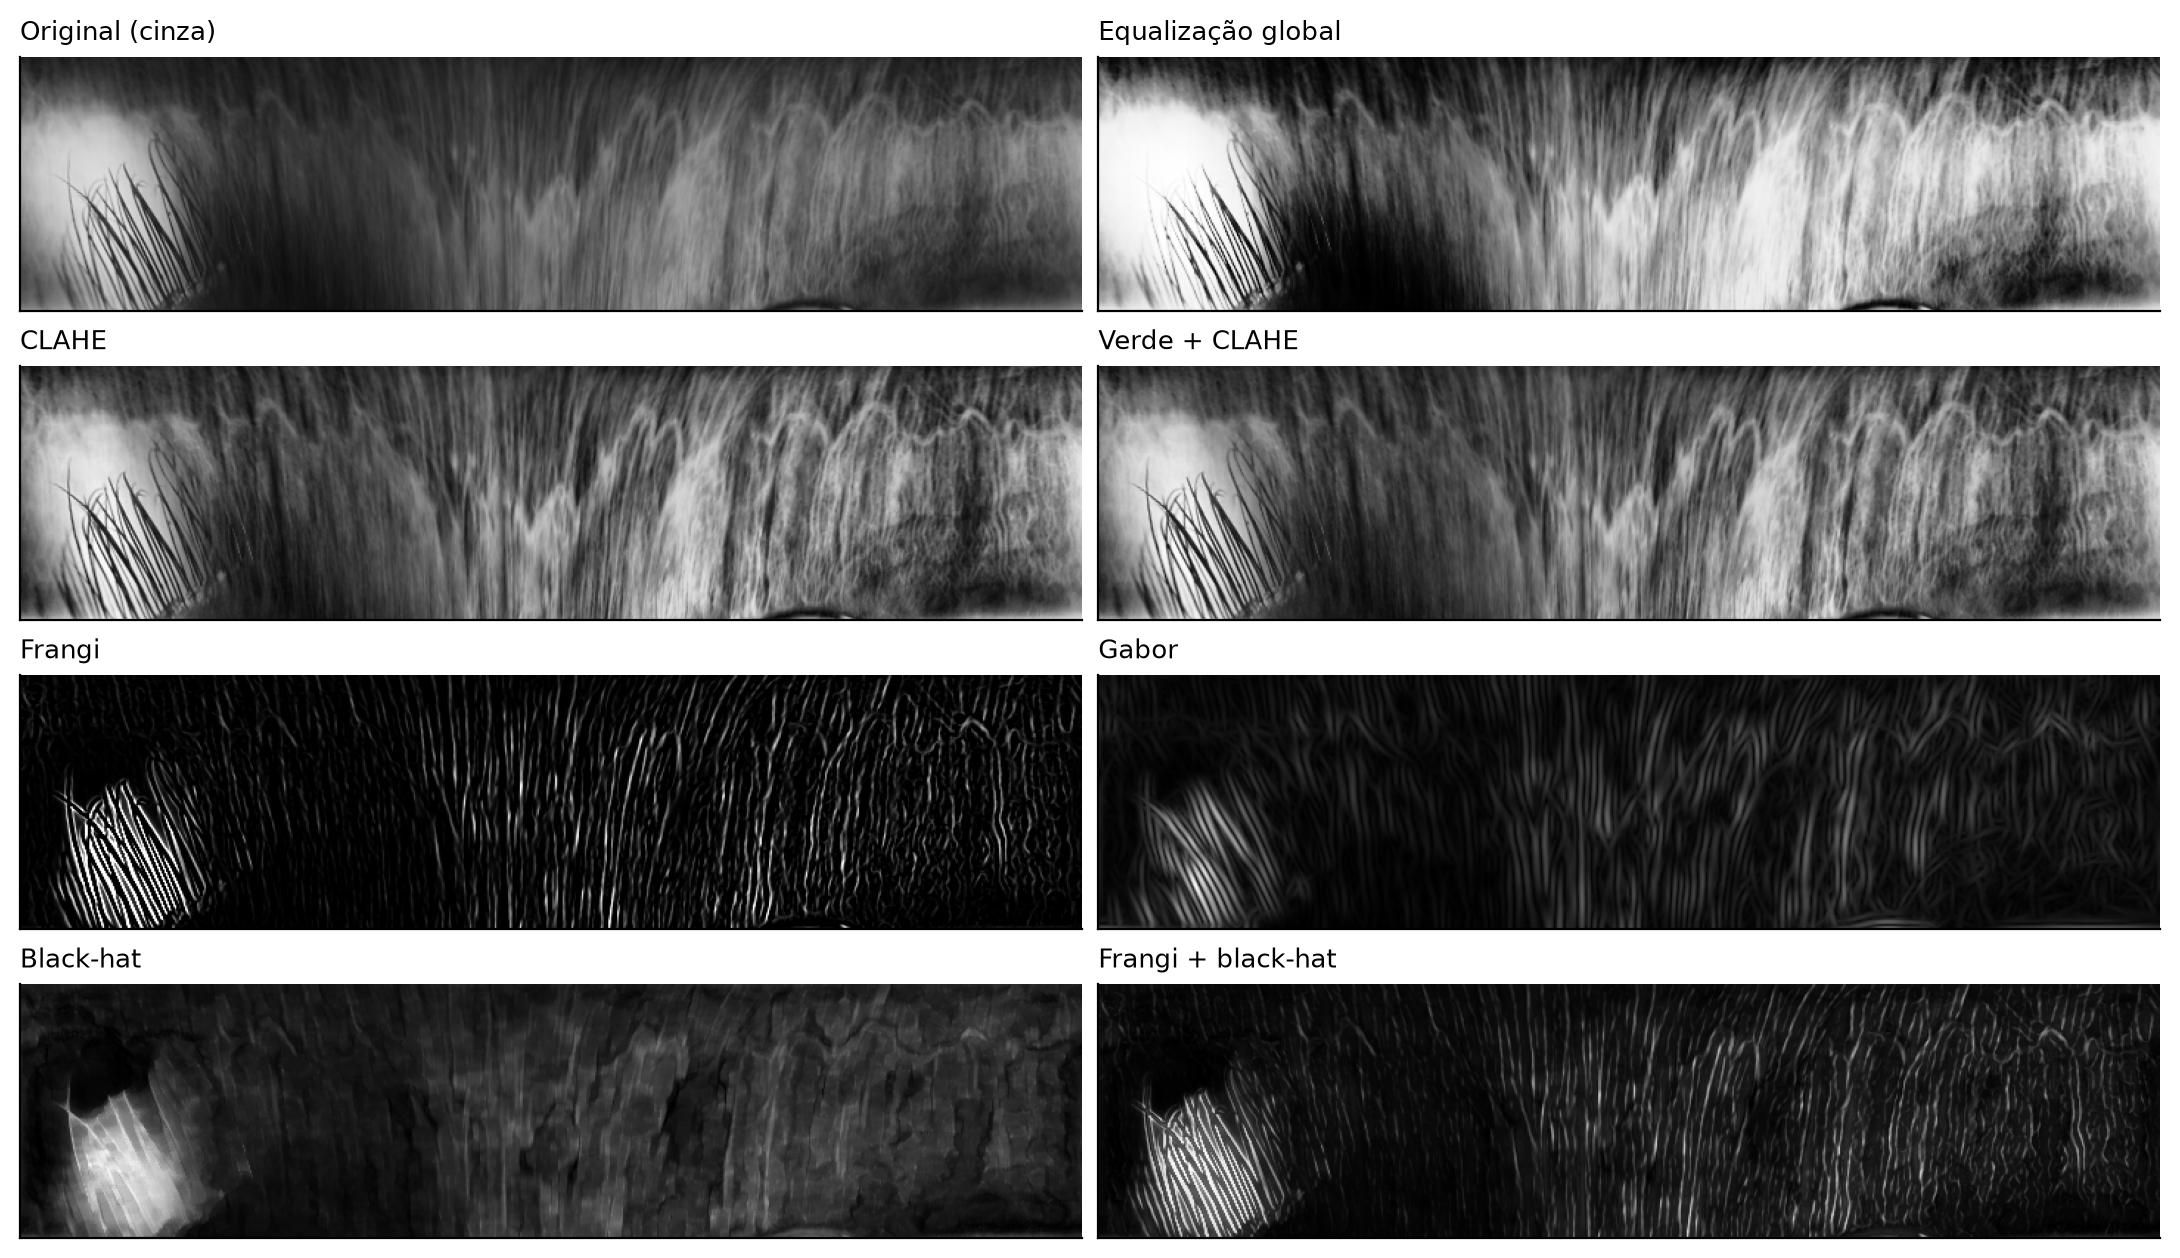
\includegraphics[width=\textwidth]{representacoes_faixa_novak.png}
  \par\medskip
  \footnotesize Fonte: elaborada pelo autor a partir da fotografia de
  \citet{Novak2005}, sob a mesma licença CC BY-SA 2.5.
\end{figure}

\begin{figure}[htbp]
  \centering
  \caption{Mapa de Frangi da faixa e vetor de pixels correspondente}
  \label{fig:vetorpixels}
  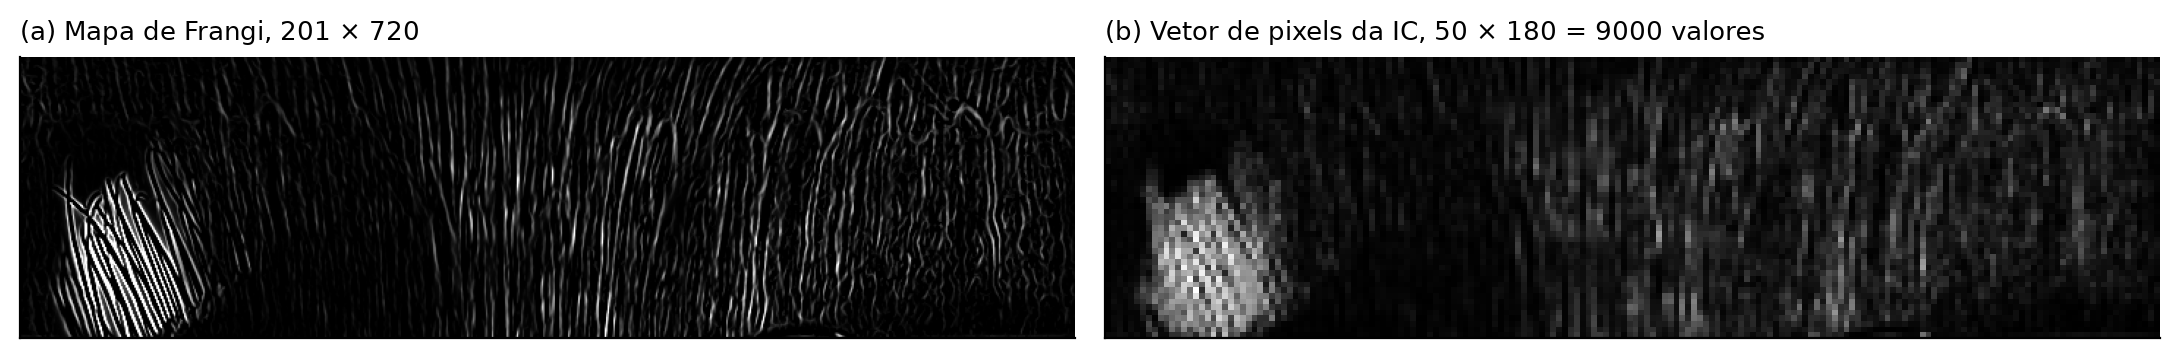
\includegraphics[width=\textwidth]{vetor_pixels_frangi_novak.png}
  \par\medskip
  \footnotesize Fonte: elaborada pelo autor a partir da fotografia de
  \citet{Novak2005}, sob a mesma licença CC BY-SA 2.5.
\end{figure}

\secao{Imagens realçadas como entrada do pipeline}
\label{sec:grade}

A Figura~\ref{fig:grade} resume as 120 configurações no leiaute principal,
\texttt{personBase\_invert}. O padrão depende do conjunto de descritores. Com
os \textbf{pixels}, ou seja, quando o classificador recebe a própria imagem,
os quatro realces superam a imagem original em \val{pix-vitorias} das 20
combinações de filtro e classificador.
A AB média sobre os classificadores passa de \val{media-pixels-original}
(original) para \val{media-pixels-frangi} (Frangi), \val{media-pixels-gabor}
(Gabor), \val{media-pixels-blackhat} (\bh) e \val{media-pixels-vessel}
(Frangi com \bh). As maiores AB com pixels vêm de Frangi com \bh{} e RF
(\val{ab-pixels-vessel-RF}), Frangi com RF (\val{ab-pixels-frangi-RF}) e \bh{}
com MLP (\val{ab-pixels-blackhat-MLP}, com a maior AUC do conjunto,
\val{auc-pixels-blackhat-MLP}). A ablação mostra que a diferença não vem do
pré-processamento comum: o canal verde com CLAHE, sem filtro, fica em
\val{media-pixels-verde_clahe}, praticamente igual à original. As
Seções~\ref{sec:replicacao} a \ref{sec:recorte} verificam o que essa
diferença representa.

Com a \textbf{textura}, a situação se inverte: a imagem original e a
equalização global são as melhores entradas (AB média
\val{media-textura-original} e \val{media-textura-histograma}, com até
\val{ab-textura-original-RF} na RF com a original), e os realces ficam entre
\val{textura-filtros-min} e \val{textura-filtros-max}. No conjunto
\textbf{padrão da IC}, que reúne pixels e textura, os realces ficam pouco
acima da original em média (\val{media-ic-original} contra valores entre
\val{ic-filtros-min} e \val{ic-filtros-max}), mas a melhor combinação
isolada desse conjunto continua sendo a imagem original com AdaBoost (AB
\val{ab-ic-original-AdaBoost}). As tabelas completas, com a AUC de cada
configuração, estão no Apêndice~\ref{ap:tabelas}.

\begin{figure}[htbp]
  \centering
  \caption{Acurácia balanceada média das 120 configurações
  (\texttt{personBase\_invert}, 50 \emph{folds})}
  \label{fig:grade}
  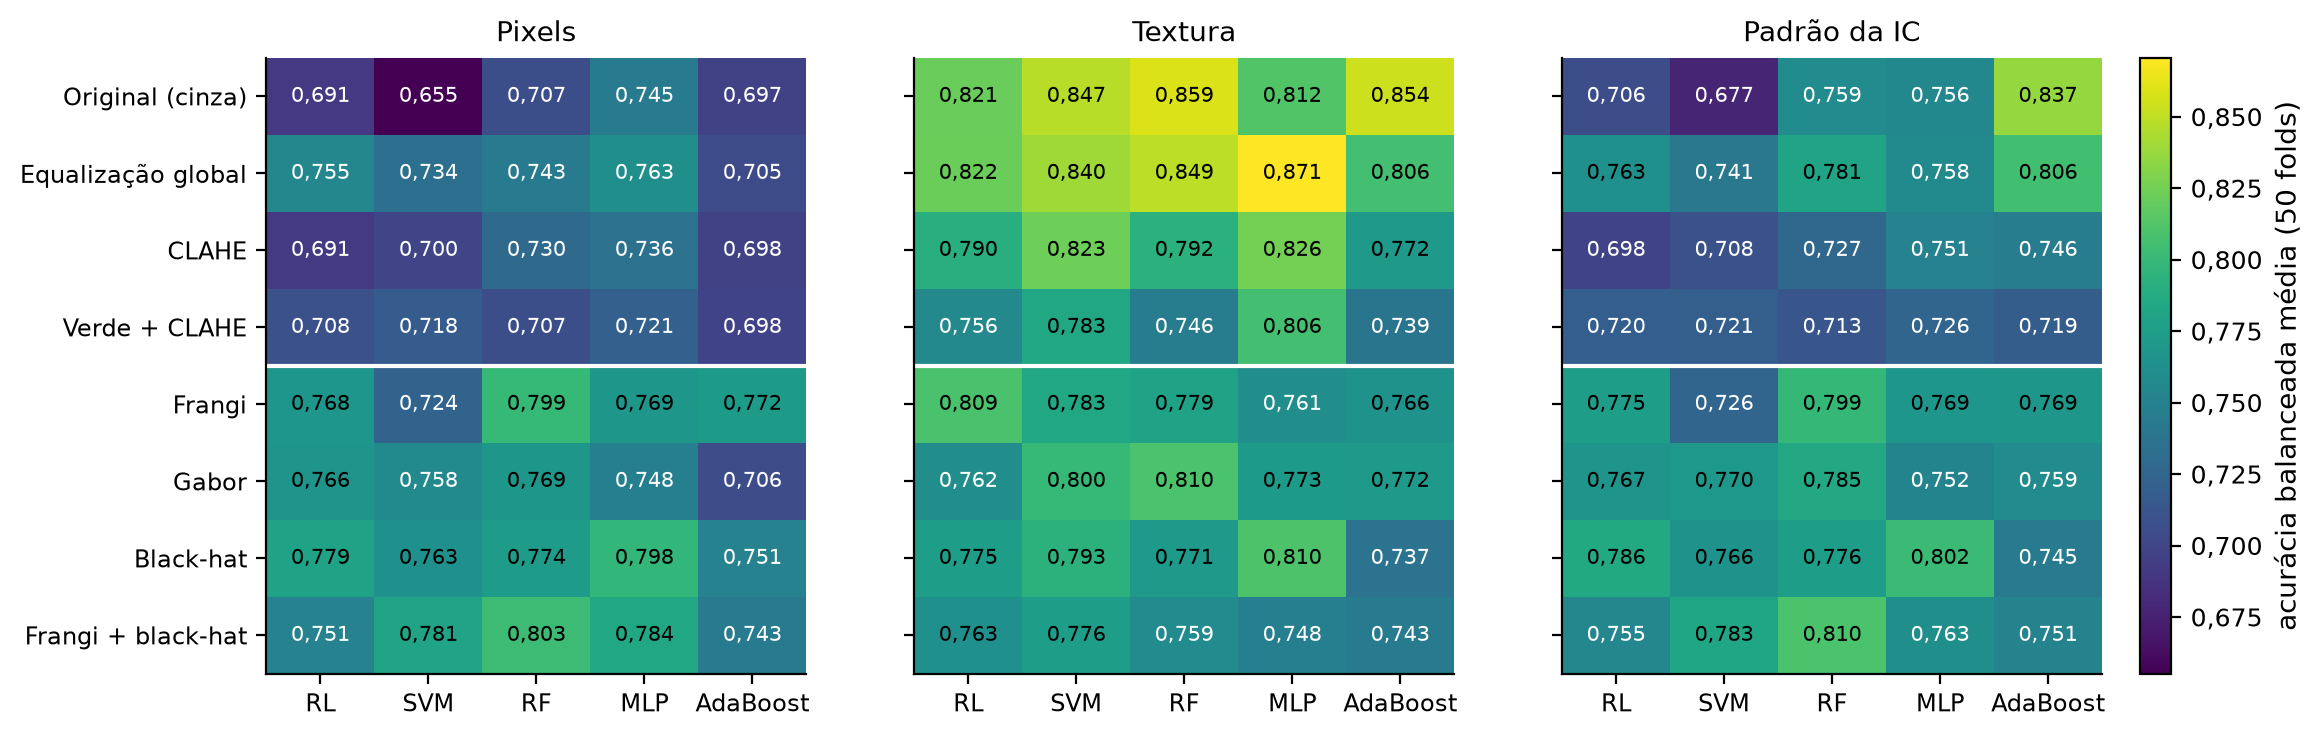
\includegraphics[width=\textwidth]{grade_acuracia_balanceada.png}
  \par\medskip
  \footnotesize Fonte: elaborada pelo autor. A linha branca separa as linhas
  de base e a ablação (acima) dos realces (abaixo).
\end{figure}

A Tabela~\ref{tab:efeito} quantifica o efeito de trocar a entrada, com a
média sobre os classificadores em cada \emph{fold}. Com pixels, todos os
realces têm diferença positiva, de \val{ef-pixels-gabor} (Gabor) a
\val{ef-pixels-blackhat} (\bh). Os intervalos de 95\% de \bh{}
($[\val{eflo-pixels-blackhat};\ \val{efhi-pixels-blackhat}]$) e de Frangi com
\bh{} ($[\val{eflo-pixels-vessel};\ \val{efhi-pixels-vessel}]$) excluem o
zero, e o de Frangi toca o zero
($[\val{eflo-pixels-frangi};\ \val{efhi-pixels-frangi}]$, \val{efp-pixels-frangi-txt}).
Depois do ajuste de Holm para as sete comparações, nenhuma diferença com
pixels permanece significativa ($p$ ajustado mínimo de
\val{efh-pixels-blackhat}), o que reflete o tamanho da base e a correção
conservadora da variância. Com textura, as diferenças são todas negativas e
duas sobrevivem ao ajuste (verde com CLAHE e Frangi com \bh).

\begin{table}[htb]
  \centering
  \caption{Diferença de acurácia balanceada em relação à imagem original
  (média dos cinco classificadores) e valor $p$ ajustado por Holm}
  \label{tab:efeito}
  \footnotesize
  % Gerado por experiments/pgc3_vascular_pipeline.py (não editar à mão).
\begin{tabular}{lccc}
\toprule
Representação & Pixels & Textura & Padrão da IC \\
\midrule
Equalização global & $+$0,041 (0,395) & $-$0,001 (0,951) & $+$0,023 (1,000) \\
CLAHE & $+$0,012 (1,000) & $-$0,038 (0,173) & $-$0,021 (1,000) \\
Verde + CLAHE & $+$0,011 (1,000) & \textbf{$-$0,073 (0,035)} & $-$0,027 (1,000) \\
\midrule
Frangi & $+$0,067 (0,257) & $-$0,059 (0,110) & $+$0,020 (1,000) \\
Gabor & $+$0,051 (0,395) & $-$0,056 (0,109) & $+$0,020 (1,000) \\
\textit{Black-hat} & $+$0,074 (0,147) & $-$0,061 (0,089) & $+$0,028 (1,000) \\
Frangi + \textit{black-hat} & $+$0,073 (0,234) & \textbf{$-$0,081 (0,014)} & $+$0,025 (1,000) \\
\bottomrule
\end{tabular}

  \par\medskip
  \footnotesize Fonte: elaborada pelo autor. Teste t pareado com a correção
  de Nadeau e Bengio sobre 50 \emph{folds}; em negrito, $p$ ajustado menor que
  0,05.
\end{table}

O teste de Friedman confirma que as representações diferem quando se
consideram os 15 blocos ($\chi^2_F=\val{fr-chi}$, \val{fr-p-txt};
$F_F=\val{fr-ff}$). A Figura~\ref{fig:cd} mostra os postos médios: a
equalização global (\val{rk-histograma}), o \bh{} (\val{rk-blackhat}) e o
Frangi (\val{rk-frangi}) ocupam as primeiras posições, a original fica em
\val{rk-original} e a ablação com verde e CLAHE, em último
(\val{rk-verde_clahe}). Com a diferença crítica de Nemenyi
($\text{CD}=\val{fr-cd}$), apenas a ablação com verde e CLAHE se distingue
das representações mais bem colocadas; as diferenças entre a imagem original
e qualquer um dos realces não são significativas.

\begin{figure}[htb]
  \centering
  \caption{Postos médios de Friedman das oito representações e diferença
  crítica de Nemenyi}
  \label{fig:cd}
  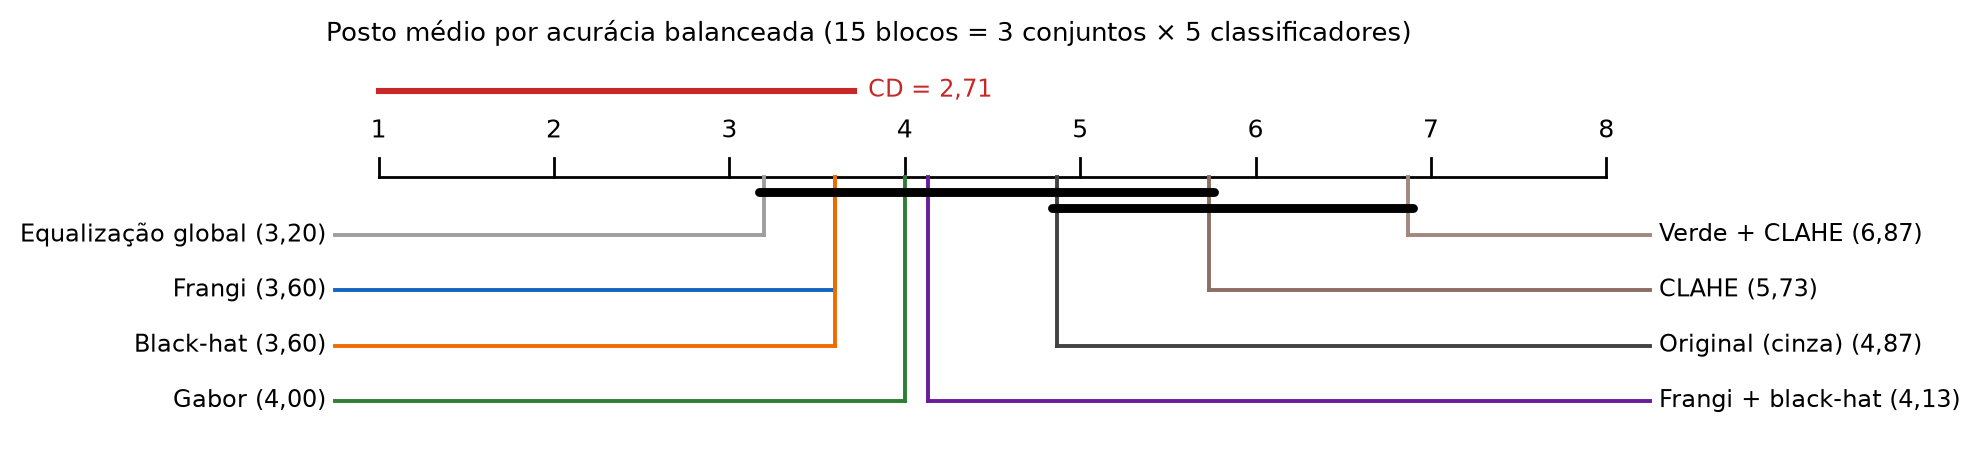
\includegraphics[width=0.95\textwidth]{diferenca_critica_ab.png}
  \par\medskip
  \footnotesize Fonte: elaborada pelo autor. Representações ligadas por uma
  barra preta não diferem segundo o teste de Nemenyi ($\alpha=0{,}05$).
\end{figure}

\secao{Desempenho acima do acaso}

No teste de permutação com o modelo pré-especificado (RL sobre os pixels),
todas as representações superam a distribuição nula
(Figura~\ref{fig:permutacao}), com \val{perm-p-txt}, o menor valor possível
com \val{prot-perm} permutações. A AB observada vai de
\val{perm-obs-verde_clahe} (verde com CLAHE) a \val{perm-obs-frangi}
(Frangi), contra uma média nula de \val{perm-nulo-media}
(desvio-padrão \val{perm-nulo-dp}). A imagem original obtém
\val{perm-obs-original}.

\begin{figure}[htb]
  \centering
  \caption{Distribuição nula da acurácia balanceada (RL sobre pixels,
  \val{prot-perm} permutações) e valor observado de cada representação}
  \label{fig:permutacao}
  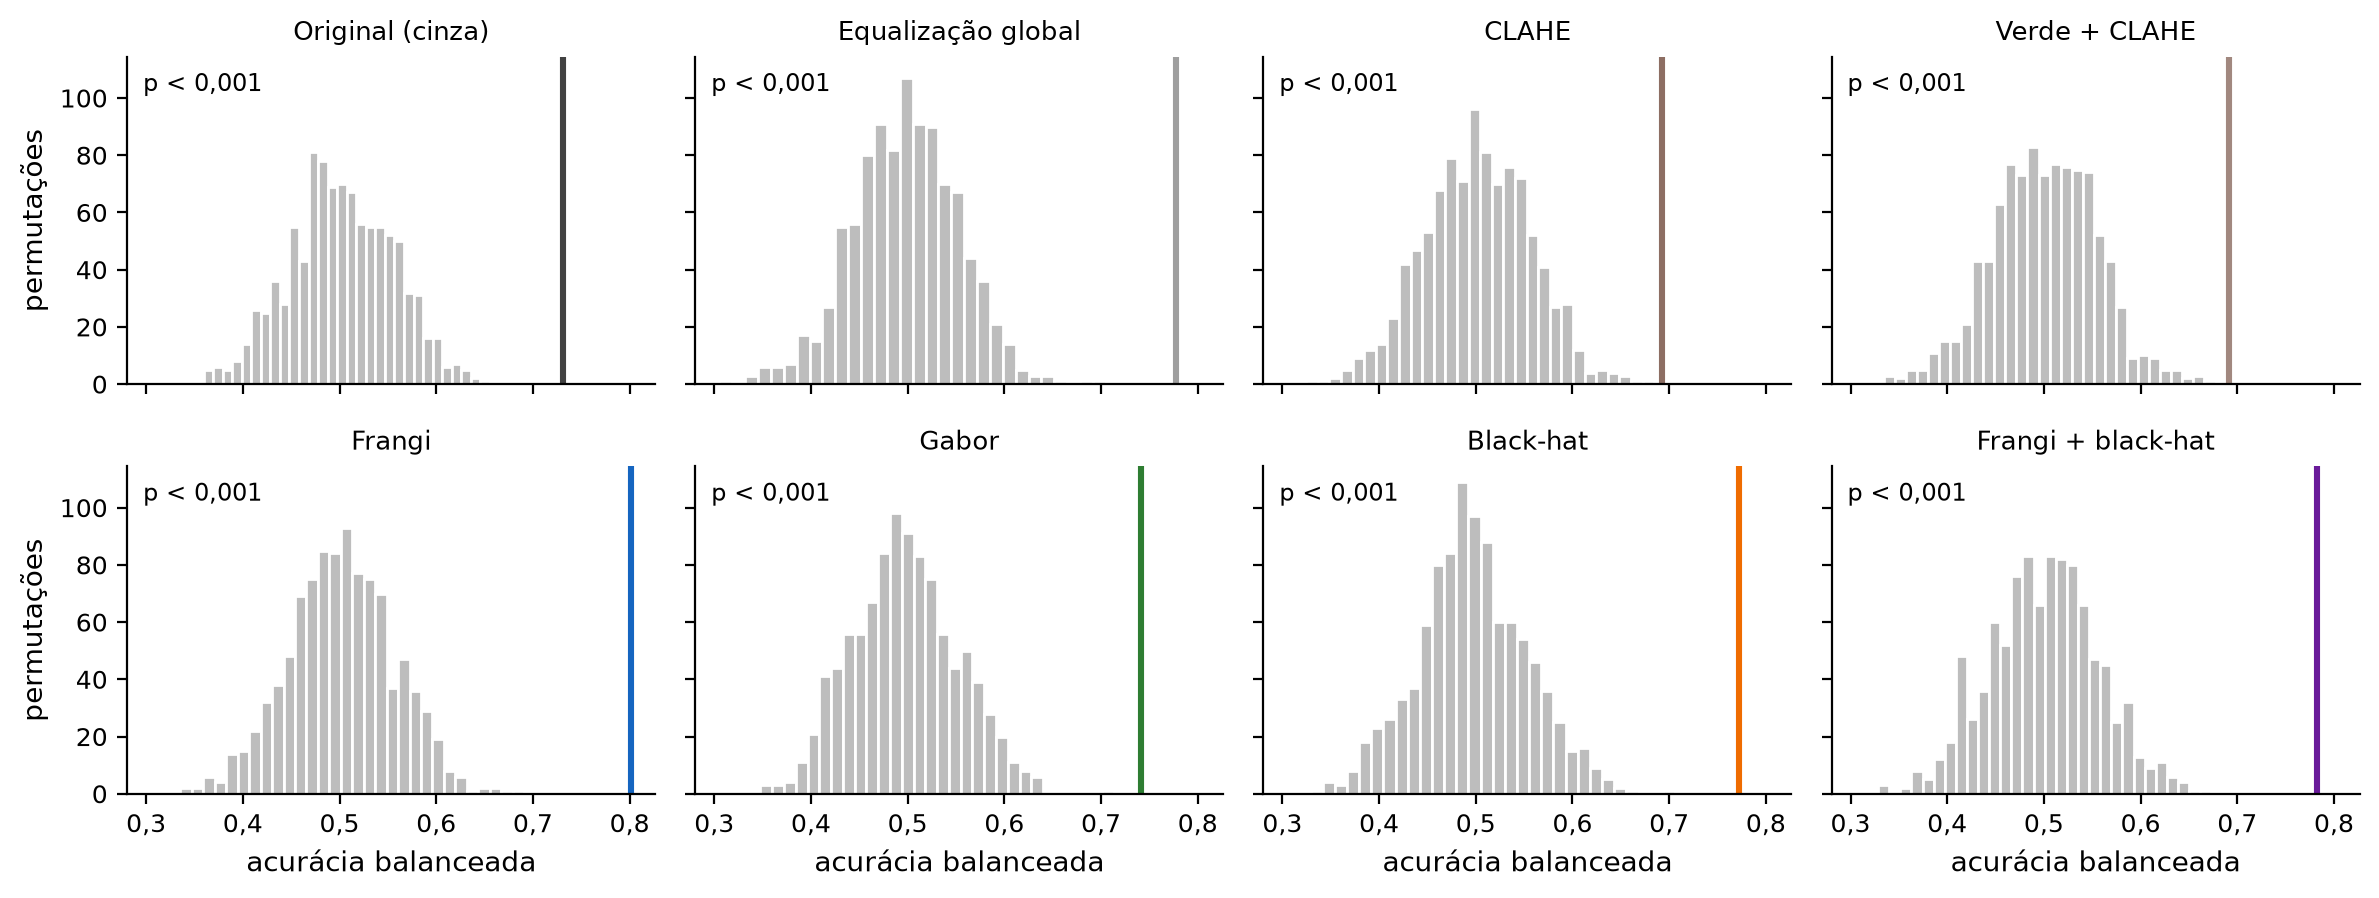
\includegraphics[width=\textwidth]{permutacao_pixels_rl.png}
  \par\medskip
  \footnotesize Fonte: elaborada pelo autor.
\end{figure}

\secao{Replicação no leiaute \texttt{personBase}}
\label{sec:replicacao}

O segundo leiaute muda a leitura dos pixels (Tabela~\ref{tab:replicacao},
Figura~\ref{fig:replicacao} e Tabela~\ref{tab:efeitopb}, no
Apêndice~\ref{ap:tabelas}). Nele, a imagem original com pixels já alcança AB
média de \val{rep-media-pixels-original}, e os realces ficam entre
\val{rep-pix-filtros-min} e \val{rep-pix-filtros-max}. Eles superam a original
em apenas \val{pb-pix-vitorias} das 20 combinações, com diferenças médias de
\val{rep-ef-pixels-blackhat} (\bh) a \val{rep-ef-pixels-gabor} (Gabor), nenhuma
significativa. O ganho com pixels do leiaute principal, portanto, não se
repete. Os descritores de textura da imagem original, ao contrário, são
estáveis entre os leiautes (\val{media-textura-original} e
\val{rep-media-textura-original}). A correlação de Spearman entre as AB médias
das 120 configurações nos dois leiautes é \val{rep-spearman}, mas a correlação
entre os postos das oito representações é de apenas \val{rep-spearman-rank}: a
ordem entre as representações não se sustenta de uma amostra para a outra.

\begin{table}[htb]
  \centering
  \caption{Replicação: acurácia balanceada média sobre os 15 blocos e posto de
  Friedman nos dois leiautes}
  \label{tab:replicacao}
  \footnotesize
  % Gerado por experiments/pgc3_vascular_pipeline.py (não editar à mão).
\begin{tabular}{lcccc}
\toprule
\multirow{2}{*}{Representação} & \multicolumn{2}{c}{\texttt{personBase\_invert}} & \multicolumn{2}{c}{\texttt{personBase}} \\
\cmidrule(lr){2-3}\cmidrule(lr){4-5}
 & AB média & Posto & AB média & Posto \\
\midrule
Original (cinza) & 0,762 & 4,87 & 0,816 & 3,47 \\
Equalização global & 0,782 & 3,20 & 0,815 & 3,60 \\
CLAHE & 0,746 & 5,73 & 0,797 & 4,93 \\
Verde + CLAHE & 0,732 & 6,87 & 0,794 & 5,47 \\
\midrule
Frangi & 0,771 & 3,60 & 0,802 & 4,13 \\
Gabor & 0,766 & 4,00 & 0,812 & 3,53 \\
\textit{Black-hat} & 0,775 & 3,60 & 0,791 & 5,80 \\
Frangi + \textit{black-hat} & 0,767 & 4,13 & 0,796 & 5,07 \\
\midrule
Friedman, $\chi^2_F$ ($p$) & \multicolumn{2}{c}{27,4 ($<$0,001)} & \multicolumn{2}{c}{15,2 (0,034)} \\
\bottomrule
\end{tabular}

  \par\medskip
  \footnotesize Fonte: elaborada pelo autor.
\end{table}

\begin{figure}[htb]
  \centering
  \caption{Replicação no leiaute \texttt{personBase}}
  \label{fig:replicacao}
  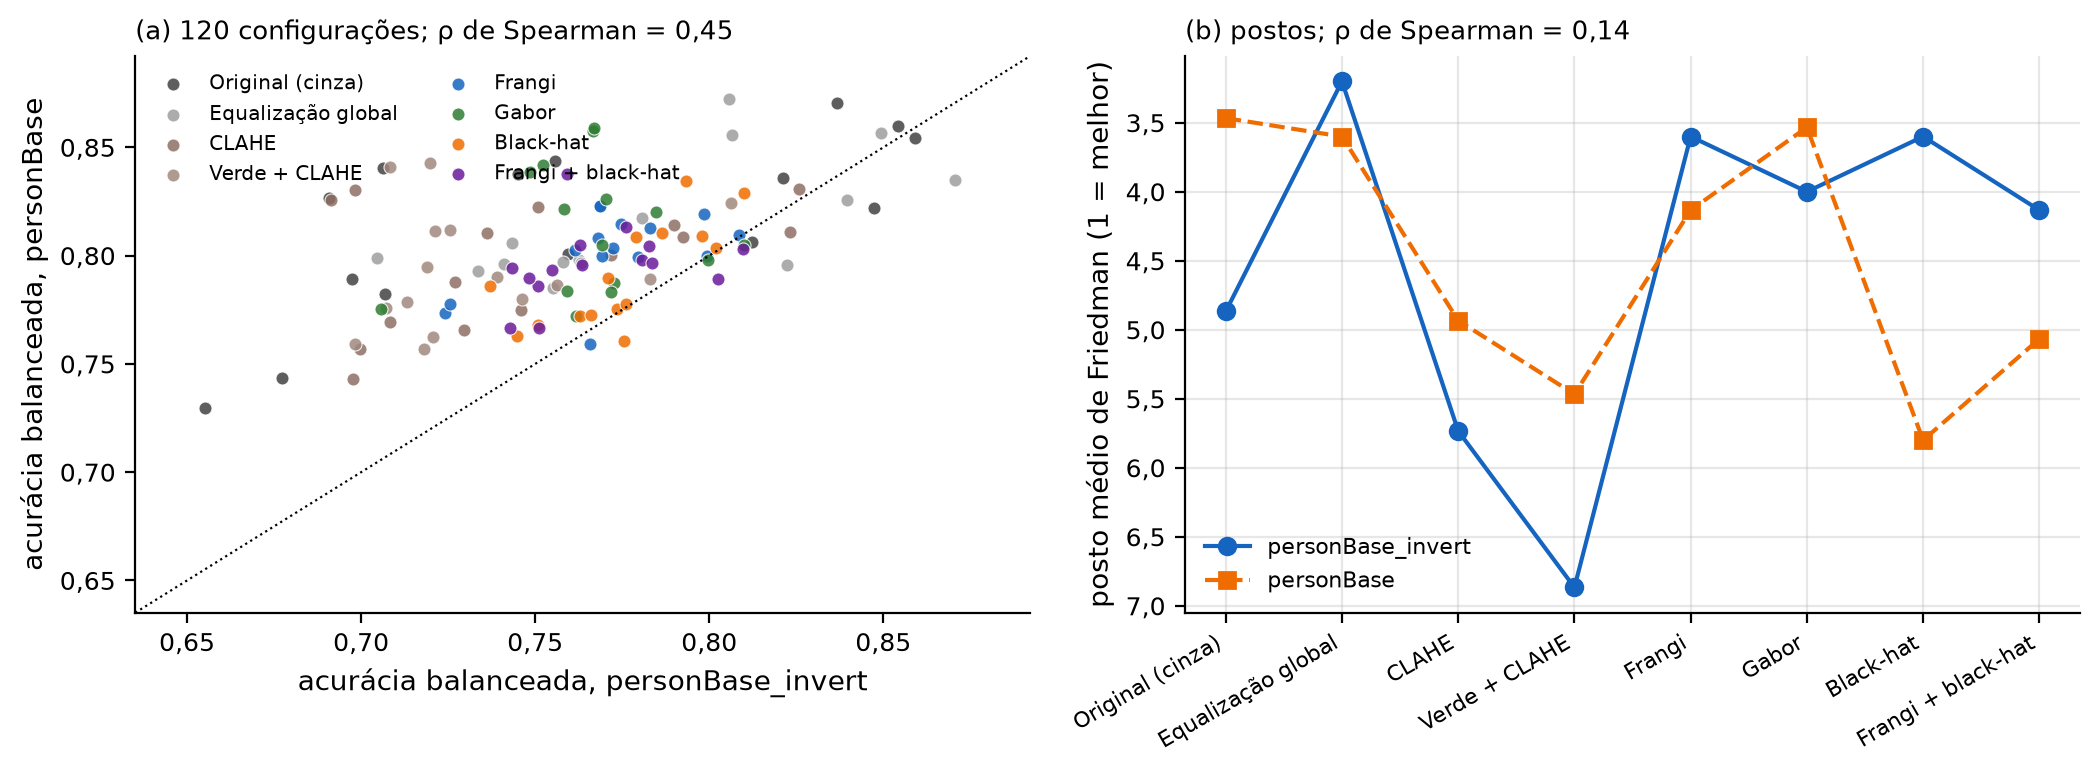
\includegraphics[width=\textwidth]{replicacao_personbase.png}
  \par\medskip
  \footnotesize Fonte: elaborada pelo autor.
\end{figure}

\secao{O espelhamento das faixas explica a diferença entre os leiautes}
\label{sec:espelhamento}

Os dois leiautes diferem num ponto de construção: no principal, as faixas do
olho direito foram espelhadas. Quando essas faixas são devolvidas à
orientação original (Tabela~\ref{tab:desespelhado} e
Figura~\ref{fig:desespelhado}), a imagem original com pixels passa de
\val{media-pixels-original} para \val{des-original}
(diferença de \val{des-mud-original}; \val{des-mudp-original-txt}) e o CLAHE, de
\val{media-pixels-clahe} para \val{des-clahe} (\val{des-mudp-clahe-txt}),
enquanto os realces quase não mudam (Frangi, \val{des-mud-frangi}; \bh,
\val{des-mud-blackhat}). Depois do desespelhamento, a vantagem dos realces
sobre a original cai para \val{des-ef-frangi} (Frangi) a \val{des-ef-vessel}
(Frangi com \bh), sem significância após o ajuste de Holm. O mecanismo é
direto: o espelhamento leva o ângulo $\theta$ a $180^\circ-\theta$ e troca os
lados direito e esquerdo da imagem em metade das faixas. Padrões de baixa
frequência ligados à câmera e à iluminação, como gradientes de luz e
reflexos, ficam do mesmo lado em todas as fotografias; o espelhamento inverte
a posição desses padrões nas faixas do olho direito, e o vetor de pixels, que
guarda a posição angular de cada valor, passa a ver duas populações
desalinhadas. Os realces descartam esses padrões e por isso são pouco
afetados. A vantagem dos realces no leiaute principal vem, em grande parte, de
uma fragilidade da representação original diante do espelhamento, e não de
informação adicional extraída pelos filtros.

\begin{table}[htb]
  \centering
  \caption{Acurácia balanceada média com pixels antes e depois de desfazer o
  espelhamento, e no leiaute \texttt{personBase}}
  \label{tab:desespelhado}
  \footnotesize
  \resizebox{\textwidth}{!}{% Gerado por experiments/pgc3_vascular_pipeline.py (não editar à mão).
\begin{tabular}{lcccc}
\toprule
\multirow{2}{*}{Representação} & \multicolumn{3}{c}{AB média com pixels} & \multirow{2}{*}{\makecell{$\Delta$ ao desfazer\\o espelhamento ($p$)}} \\
\cmidrule(lr){2-4}
 & \makecell{\texttt{personBase\_invert}\\(espelhado)} & \makecell{\texttt{personBase\_invert}\\(desespelhado)} & \texttt{personBase} & \\
\midrule
Original (cinza) & 0,699 & 0,752 & 0,793 & $+$0,053 (0,064) \\
Equalização global & 0,740 & 0,778 & 0,796 & $+$0,038 (0,179) \\
CLAHE & 0,711 & 0,772 & 0,780 & $+$0,062 (0,017) \\
Verde + CLAHE & 0,711 & 0,761 & 0,789 & $+$0,050 (0,087) \\
\midrule
Frangi & 0,767 & 0,773 & 0,802 & $+$0,007 (0,747) \\
Gabor & 0,750 & 0,779 & 0,820 & $+$0,029 (0,202) \\
\textit{Black-hat} & 0,773 & 0,774 & 0,787 & $+$0,001 (0,968) \\
Frangi + \textit{black-hat} & 0,772 & 0,787 & 0,787 & $+$0,015 (0,481) \\
\bottomrule
\end{tabular}
}
  \par\medskip
  \footnotesize Fonte: elaborada pelo autor. $\Delta$: diferença pareada,
  \emph{fold} a \emph{fold}, entre as versões desespelhada e espelhada (teste
  t corrigido).
\end{table}

\begin{figure}[htb]
  \centering
  \caption{Efeito de desfazer o espelhamento das faixas do olho direito}
  \label{fig:desespelhado}
  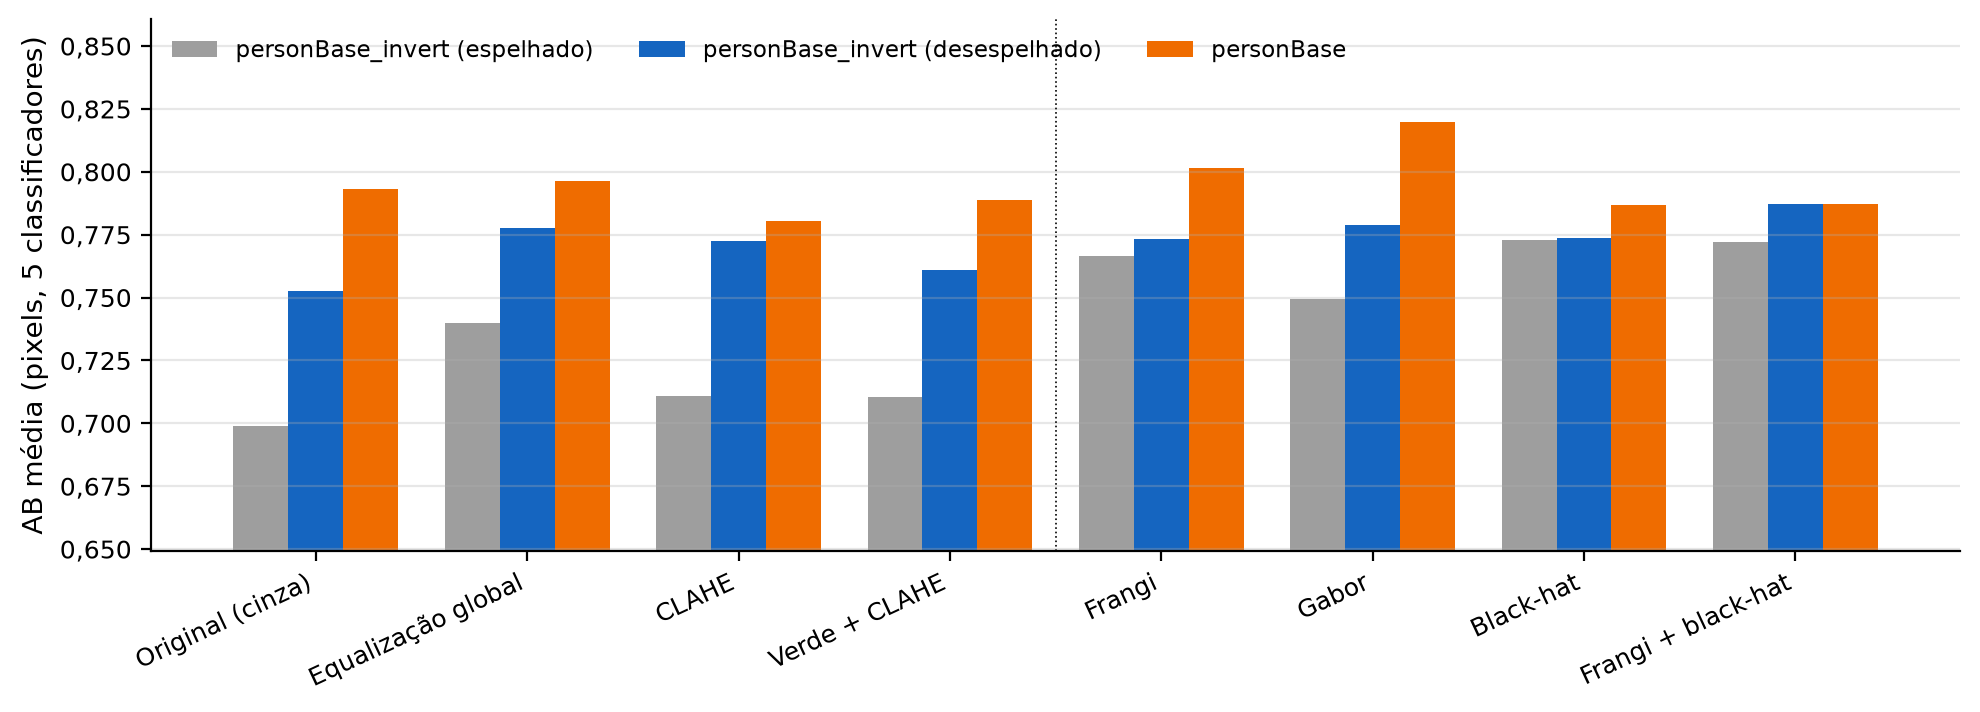
\includegraphics[width=\textwidth]{desespelhamento.png}
  \par\medskip
  \footnotesize Fonte: elaborada pelo autor.
\end{figure}

\secao{Estroma ou bordas: onde está o sinal}
\label{sec:recorte}

A Figura~\ref{fig:mapas} mostra o $d$ de Cohen por pixel no leiaute
principal. Na imagem original, apenas \val{map-frac-original}\% dos pixels
mantêm diferença significativa após o controle da FDR; com os realces, a
fração sobe para \val{map-frac-frangi}\% (Frangi), \val{map-frac-gabor}\%
(Gabor), \val{map-frac-vessel}\% (Frangi com \bh) e \val{map-frac-blackhat}\%
(\bh). A localização, porém, varia: nos mapas de Frangi e de Frangi com \bh,
as diferenças se concentram numa faixa junto ao limbo ($r$ próximo de 1); no
Gabor, junto à margem pupilar ($r$ próximo de 0); e o \bh{} mostra, além da
faixa límbica, regiões no próprio estroma.

\begin{figure}[htbp]
  \centering
  \caption{Diferença entre classes por pixel ($d$ de Cohen, diabetes menos
  controle) em seis representações}
  \label{fig:mapas}
  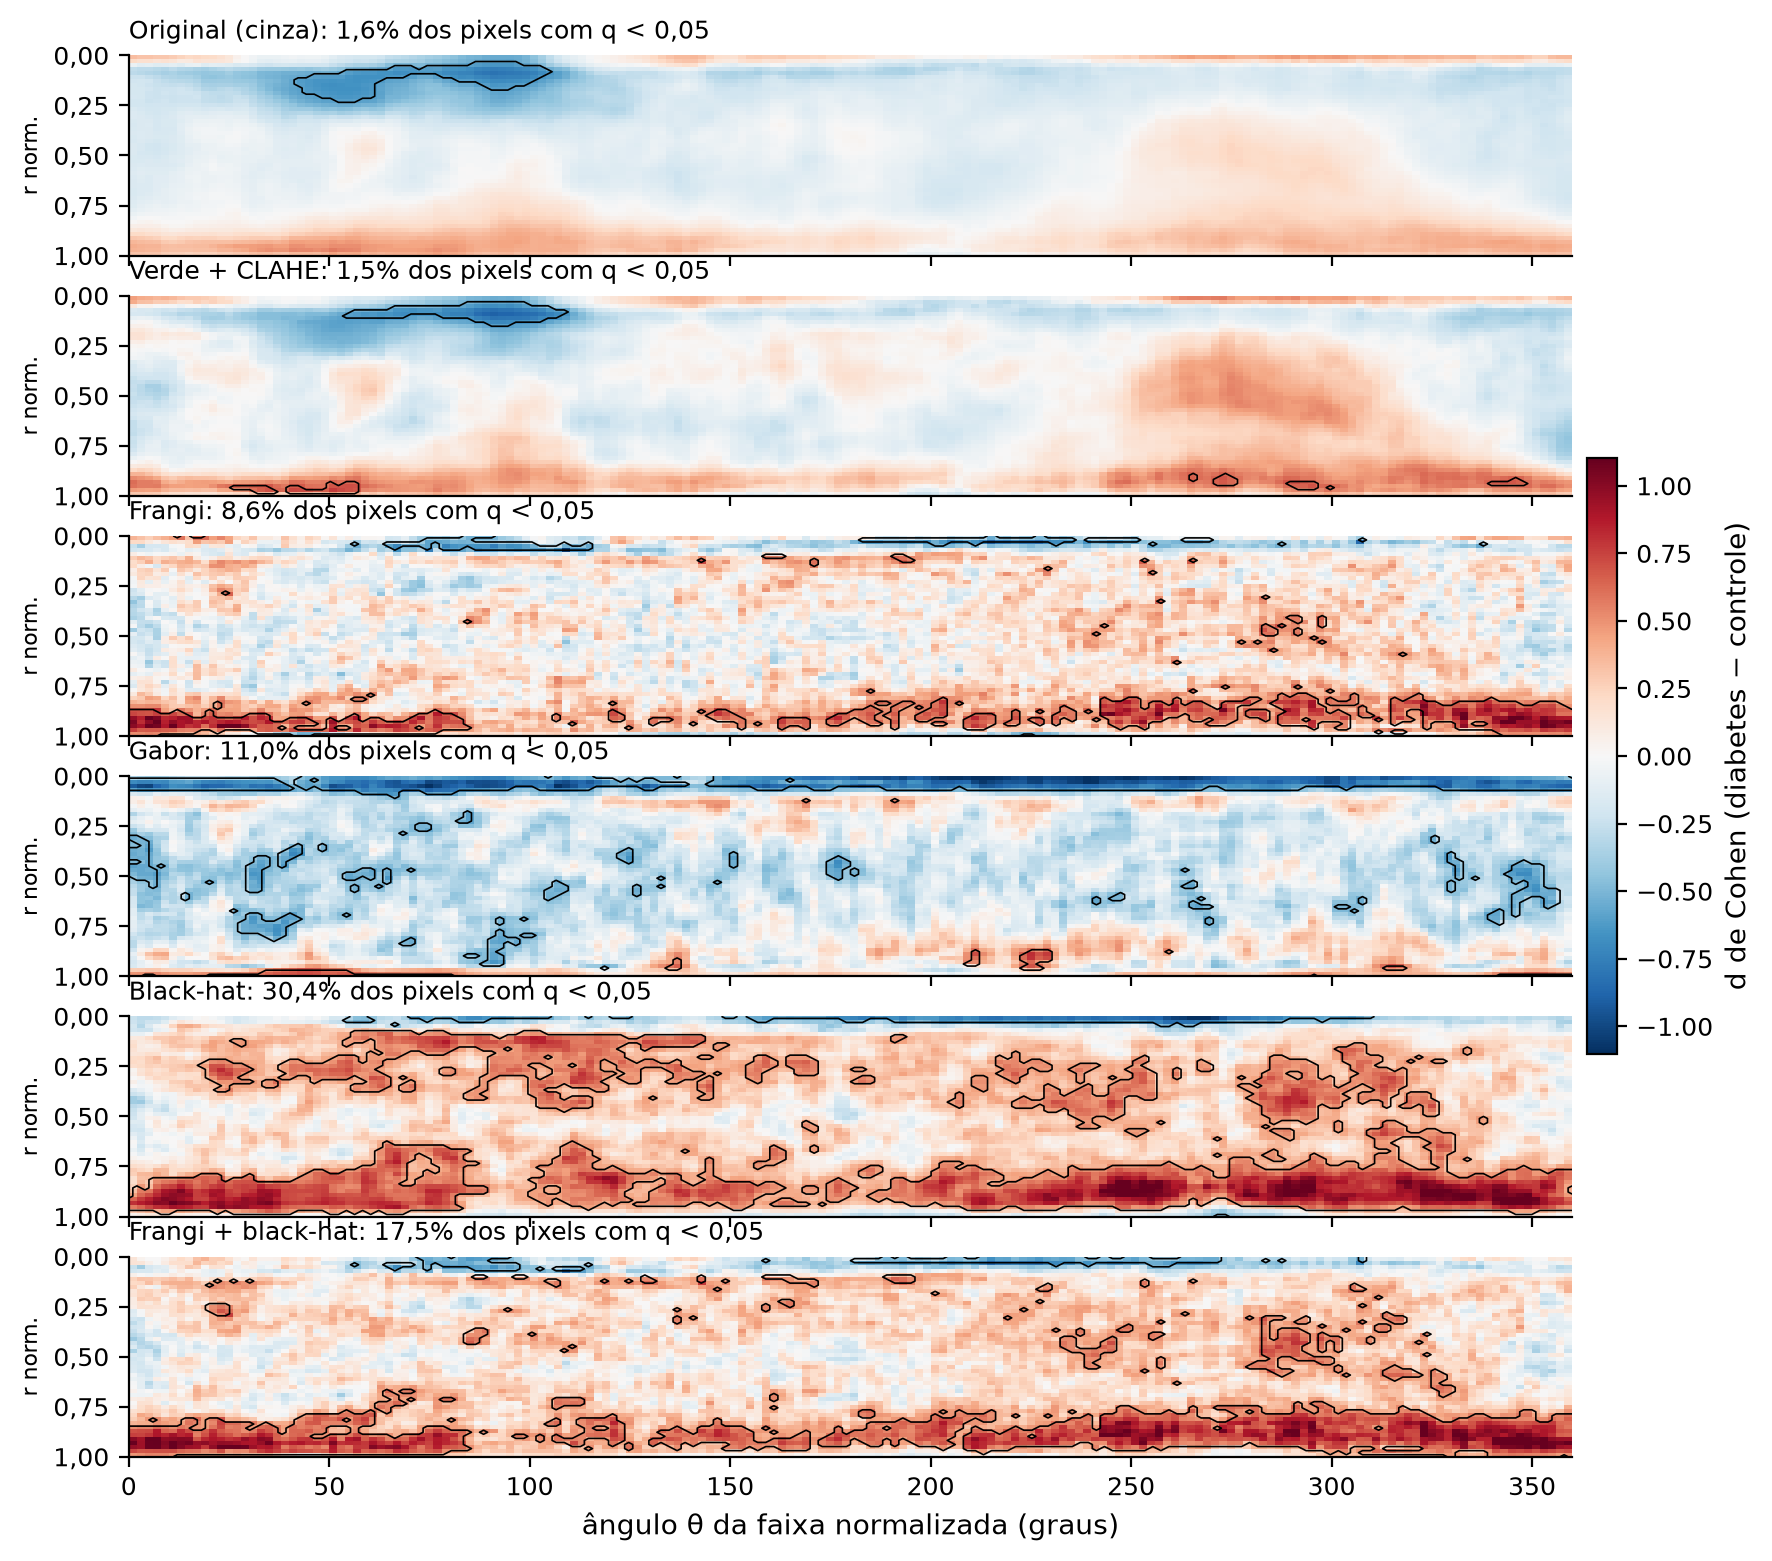
\includegraphics[width=\textwidth]{mapas_d_cohen.png}
  \par\medskip
  \footnotesize Fonte: elaborada pelo autor. Contornos pretos: pixels com
  $q<0{,}05$ após o controle da FDR. Mapas agregados; nenhuma imagem
  individual da base é mostrada.
\end{figure}

O recorte radial (Tabela~\ref{tab:recorte} e Figura~\ref{fig:recorte})
confirma essa leitura. Com apenas o estroma, todas as representações perdem
desempenho: a original fica em \val{rec-estroma-original} e os realces, entre
\val{rec-estroma-filtros-min} e \val{rec-estroma-filtros-max}, superando a
original em \val{rec-vit-estroma} das 20 combinações e sem diferença
significativa. O \bh{}, coerente com as regiões de estroma vistas no seu mapa,
é o único realce que mantém AB em torno de 0,70 nessa região
(\val{rec-estroma-blackhat}), mas sua vantagem sobre a original
(\val{rec-ef-estroma-blackhat}) não sobrevive ao ajuste de Holm
(\val{rec-efh-estroma-blackhat-txt}).
Com apenas as bordas, os realces alcançam entre \val{rec-bordas-filtros-min} e
\val{rec-bordas-filtros-max}, contra \val{rec-bordas-original} da original, e
a superam em \val{rec-vit-bordas} das 20 combinações. Para Frangi
(\val{rec-ef-bordas-frangi}; $p$ ajustado \val{rec-efh-bordas-frangi}), Gabor
(\val{rec-ef-bordas-gabor}; \val{rec-efh-bordas-gabor}) e Frangi com \bh{}
(\val{rec-ef-bordas-vessel}; \val{rec-efh-bordas-vessel}), essa é a única
vantagem dos realces que sobrevive ao ajuste de Holm em todo o estudo. O sinal
que os realces evidenciam nesta base está, portanto, nas transições da pupila
e do limbo, regiões que dependem da segmentação, da nitidez e das condições de
aquisição, e não no estroma vascularizado.

\begin{table}[htb]
  \centering
  \caption{Acurácia balanceada média com pixels por região radial da faixa e
  diferença em relação à original}
  \label{tab:recorte}
  \footnotesize
  % Gerado por experiments/pgc3_vascular_pipeline.py (não editar à mão).
\begin{tabular}{lccccc}
\toprule
\multirow{2}{*}{Representação} & Faixa inteira & \multicolumn{2}{c}{Só estroma} & \multicolumn{2}{c}{Só bordas} \\
\cmidrule(lr){3-4}\cmidrule(lr){5-6}
 & AB & AB & $\Delta$ ($p$ Holm) & AB & $\Delta$ ($p$ Holm) \\
\midrule
Original (cinza) & 0,699 & 0,632 & -- & 0,704 & -- \\
Equalização global & 0,740 & 0,659 & $+$0,027 (1,000) & 0,751 & $+$0,047 (0,319) \\
CLAHE & 0,711 & 0,638 & $+$0,006 (1,000) & 0,725 & $+$0,021 (0,795) \\
Verde + CLAHE & 0,711 & 0,635 & $+$0,004 (1,000) & 0,711 & $+$0,007 (0,795) \\
\midrule
Frangi & 0,767 & 0,609 & $-$0,022 (1,000) & 0,814 & \textbf{$+$0,110 (0,002)} \\
Gabor & 0,750 & 0,597 & $-$0,035 (1,000) & 0,811 & \textbf{$+$0,107 (0,003)} \\
\textit{Black-hat} & 0,773 & 0,702 & $+$0,070 (0,207) & 0,779 & $+$0,075 (0,080) \\
Frangi + \textit{black-hat} & 0,772 & 0,642 & $+$0,011 (1,000) & 0,794 & \textbf{$+$0,090 (0,038)} \\
\bottomrule
\end{tabular}

  \par\medskip
  \footnotesize Fonte: elaborada pelo autor. Estroma: $r$ entre 0,10 e 0,86;
  bordas: $r<0{,}10$ ou $r>0{,}86$. $\Delta$: média dos cinco classificadores;
  teste t corrigido e ajuste de Holm; em negrito, $p$ ajustado menor que 0,05.
\end{table}

\begin{figure}[htb]
  \centering
  \caption{Acurácia balanceada média com pixels da faixa inteira, só do estroma
  e só das bordas}
  \label{fig:recorte}
  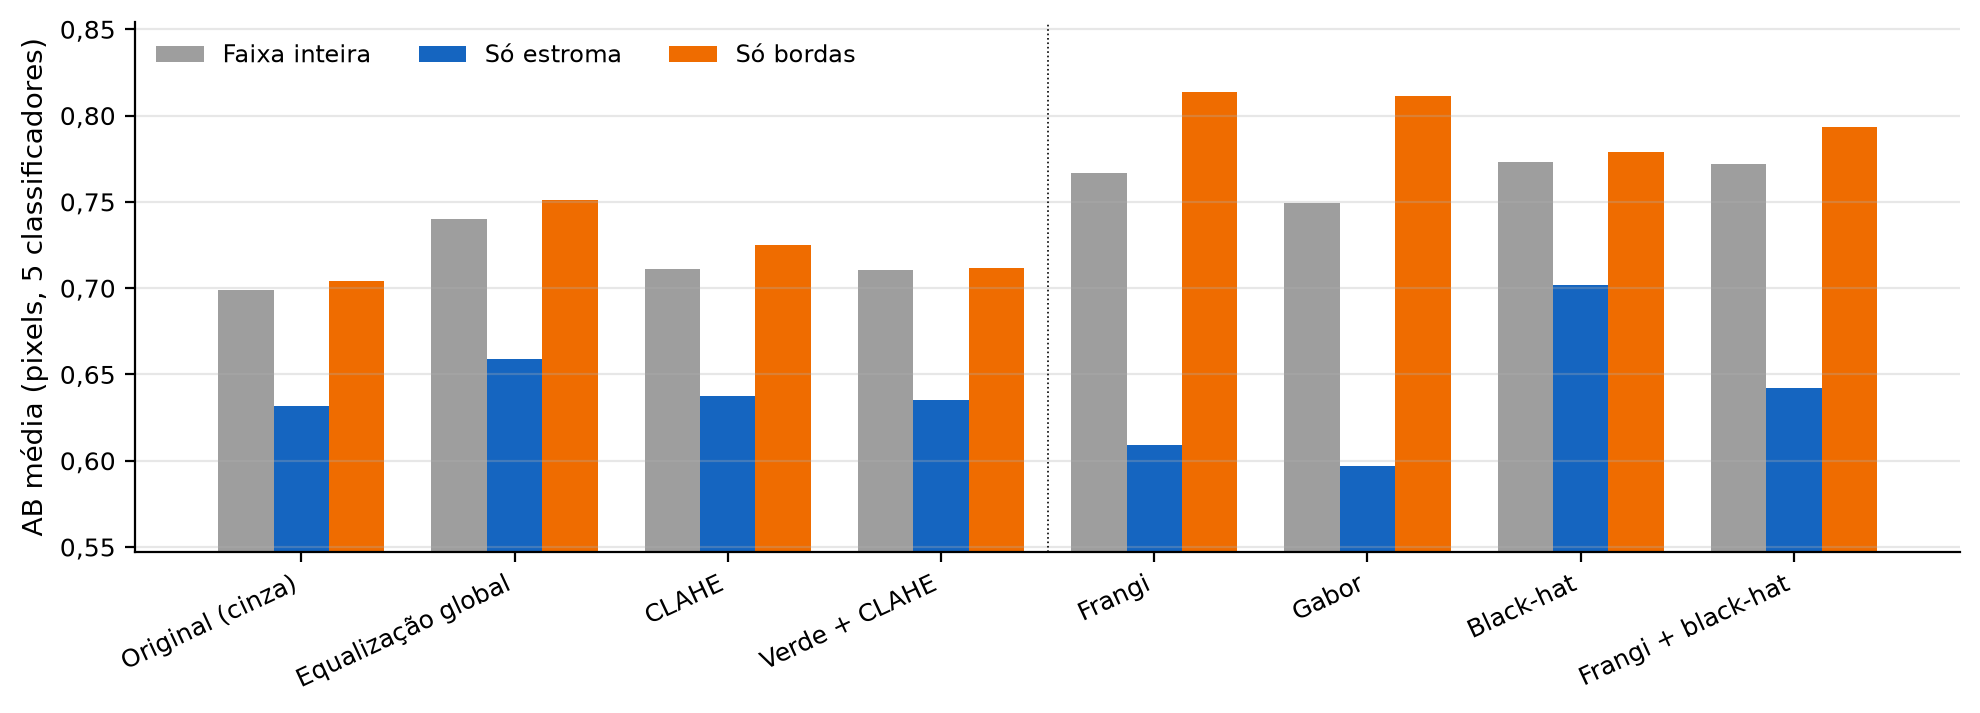
\includegraphics[width=\textwidth]{recorte_radial.png}
  \par\medskip
  \footnotesize Fonte: elaborada pelo autor.
\end{figure}

\secao{Controles: atalho de cor, descritores manuais e fusão}
\label{sec:controles}

A Tabela~\ref{tab:controles} traz os três controles. As oito estatísticas
globais de cor e iluminação alcançam AB de até \val{ctl-abmax-cor}
(\val{ctl-clfmax-cor}), o que confirma que a diferença de cor média entre as
classes, encontrada na auditoria, carrega informação discriminativa por si
só. Os 13 descritores manuais de vascularização alcançam até
\val{ctl-abmax-manual} (\val{ctl-clfmax-manual}), valor da mesma ordem que o
da imagem de Frangi como entrada direta (\val{media-pixels-frangi} em média com
pixels e até \val{ab-pixels-frangi-RF} com RF). A fusão da imagem original com
a imagem realçada chega a \val{ctl-abmax-fusao_frangi} (original + Frangi,
\val{ctl-clfmax-fusao_frangi}) e \val{ctl-abmax-fusao_gabor} (original +
Gabor, \val{ctl-clfmax-fusao_gabor}), abaixo da melhor combinação do conjunto
padrão da IC com a imagem original (\val{ab-ic-original-AdaBoost}).

\begin{table}[htb]
  \centering
  \caption{Controles: acurácia balanceada (AUC entre parênteses), média de 50
  \emph{folds}}
  \label{tab:controles}
  \footnotesize
  \resizebox{\textwidth}{!}{% Gerado por experiments/pgc3_vascular_pipeline.py (não editar à mão).
\begin{tabular}{lccccc}
\toprule
Entrada & RL & SVM & RF & MLP & AdaBoost \\
\midrule
Referência: Original (cinza) (padrão da IC) & 0,706 (0,799) & 0,677 (0,765) & 0,759 (0,830) & 0,756 (0,835) & 0,837 (0,910) \\
Referência: Frangi (padrão da IC) & 0,775 (0,820) & 0,726 (0,801) & 0,799 (0,852) & 0,769 (0,818) & 0,769 (0,830) \\
Referência: Gabor (padrão da IC) & 0,767 (0,834) & 0,770 (0,838) & 0,785 (0,840) & 0,752 (0,812) & 0,759 (0,807) \\
\midrule
Cor e iluminação globais (8 valores) & 0,739 (0,777) & 0,684 (0,751) & 0,718 (0,797) & 0,769 (0,843) & 0,685 (0,743) \\
Descritores manuais de Frangi (13 valores) & 0,777 (0,845) & 0,721 (0,782) & 0,716 (0,736) & 0,733 (0,771) & 0,716 (0,776) \\
Fusão: original + Frangi (padrão da IC) & 0,771 (0,843) & 0,741 (0,803) & 0,815 (0,855) & 0,756 (0,835) & 0,807 (0,861) \\
Fusão: original + Gabor (padrão da IC) & 0,771 (0,846) & 0,752 (0,825) & 0,794 (0,860) & 0,751 (0,829) & 0,804 (0,841) \\
\bottomrule
\end{tabular}
}
  \par\medskip
  \footnotesize Fonte: elaborada pelo autor.
\end{table}

\secao{Robustez fotométrica}

A Tabela~\ref{tab:robustez} e a Figura~\ref{fig:robustez} mostram a variação
da AB quando o modelo, treinado na condição original, é testado sob
perturbações. A equalização global, o CLAHE e o Gabor são as representações
mais estáveis (variação absoluta média de \val{rob-mabs-clahe} para CLAHE,
\val{rob-mabs-gabor} para Gabor e \val{rob-mabs-histograma} para a
equalização global). A imagem original varia \val{rob-mabs-original} em média,
com quedas significativas sob escurecimento, gama 1,5 e ruído. O ruído
gaussiano reduz a AB de quase todas as representações, e os realces de Frangi
e \bh{} são os mais afetados por ele e pelo desfoque (piores quedas de
\val{rob-pior-frangi} e \val{rob-pior-blackhat}), o que é coerente com o fato
de responderem justamente às estruturas finas que essas perturbações alteram.
O Gabor, que combina oito orientações numa banda de frequências mais larga, é
o único realce sem queda significativa sob ruído.

\begin{table}[htb]
  \centering
  \caption{Variação da acurácia balanceada sob perturbações (RL, conjunto
  padrão da IC; treino na condição original)}
  \label{tab:robustez}
  \footnotesize
  \resizebox{\textwidth}{!}{% Gerado por experiments/pgc3_vascular_pipeline.py (não editar à mão).
\begin{tabular}{lcccccccc}
\toprule
Perturbação & Orig. & Eq. & CLAHE & V+CL & Frangi & Gabor & \textit{B-hat} & F+BH \\
\midrule
Brilho $-30$ & \textbf{$-$0,166} & $-$0,010 & $-$0,008 & \textbf{$-$0,173} & $-$0,072 & \textbf{$-$0,103} & $-$0,066 & $-$0,054 \\
Brilho $+30$ & $-$0,031 & 0,000 & $+$0,014 & \textbf{$-$0,173} & $-$0,002 & $+$0,005 & $-$0,007 & $+$0,004 \\
Contraste $\times0{,}7$ & $+$0,002 & $-$0,008 & $+$0,000 & $+$0,001 & $+$0,003 & $-$0,004 & $-$0,008 & $+$0,008 \\
Contraste $\times1{,}3$ & $-$0,003 & $+$0,003 & $-$0,008 & $-$0,020 & $+$0,007 & $-$0,001 & $-$0,002 & $+$0,009 \\
Gama $0{,}7$ & $+$0,003 & $+$0,000 & $+$0,003 & $-$0,021 & $+$0,001 & $-$0,014 & $-$0,006 & $+$0,016 \\
Gama $1{,}5$ & \textbf{$-$0,106} & $-$0,006 & $-$0,006 & $-$0,095 & $-$0,020 & $-$0,018 & $-$0,031 & $+$0,004 \\
Ruído ($\sigma=8$) & \textbf{$-$0,206} & \textbf{$-$0,182} & \textbf{$-$0,175} & \textbf{$-$0,182} & \textbf{$-$0,275} & $-$0,077 & \textbf{$-$0,286} & \textbf{$-$0,255} \\
Desfoque ($\sigma=1{,}5$) & $-$0,046 & $-$0,044 & $-$0,005 & \textbf{$-$0,170} & \textbf{$-$0,231} & $-$0,044 & \textbf{$-$0,146} & $-$0,079 \\
JPEG ($q=30$) & $-$0,049 & $-$0,065 & $+$0,002 & $+$0,006 & $-$0,034 & $+$0,002 & \textbf{$-$0,098} & $-$0,069 \\
\midrule
Média de $|\Delta|$ & 0,068 & 0,035 & 0,025 & 0,093 & 0,071 & 0,030 & 0,072 & 0,055 \\
\bottomrule
\end{tabular}
}
  \par\medskip
  \footnotesize Fonte: elaborada pelo autor. Em negrito, intervalo de 95\%
  corrigido que exclui o zero. Abreviaturas: Orig., original; Eq.,
  equalização global; V+CL, verde com CLAHE; B-hat, \bh; F+BH, Frangi com \bh.
\end{table}

\begin{figure}[htb]
  \centering
  \caption{Variação da acurácia balanceada sob perturbações fotométricas}
  \label{fig:robustez}
  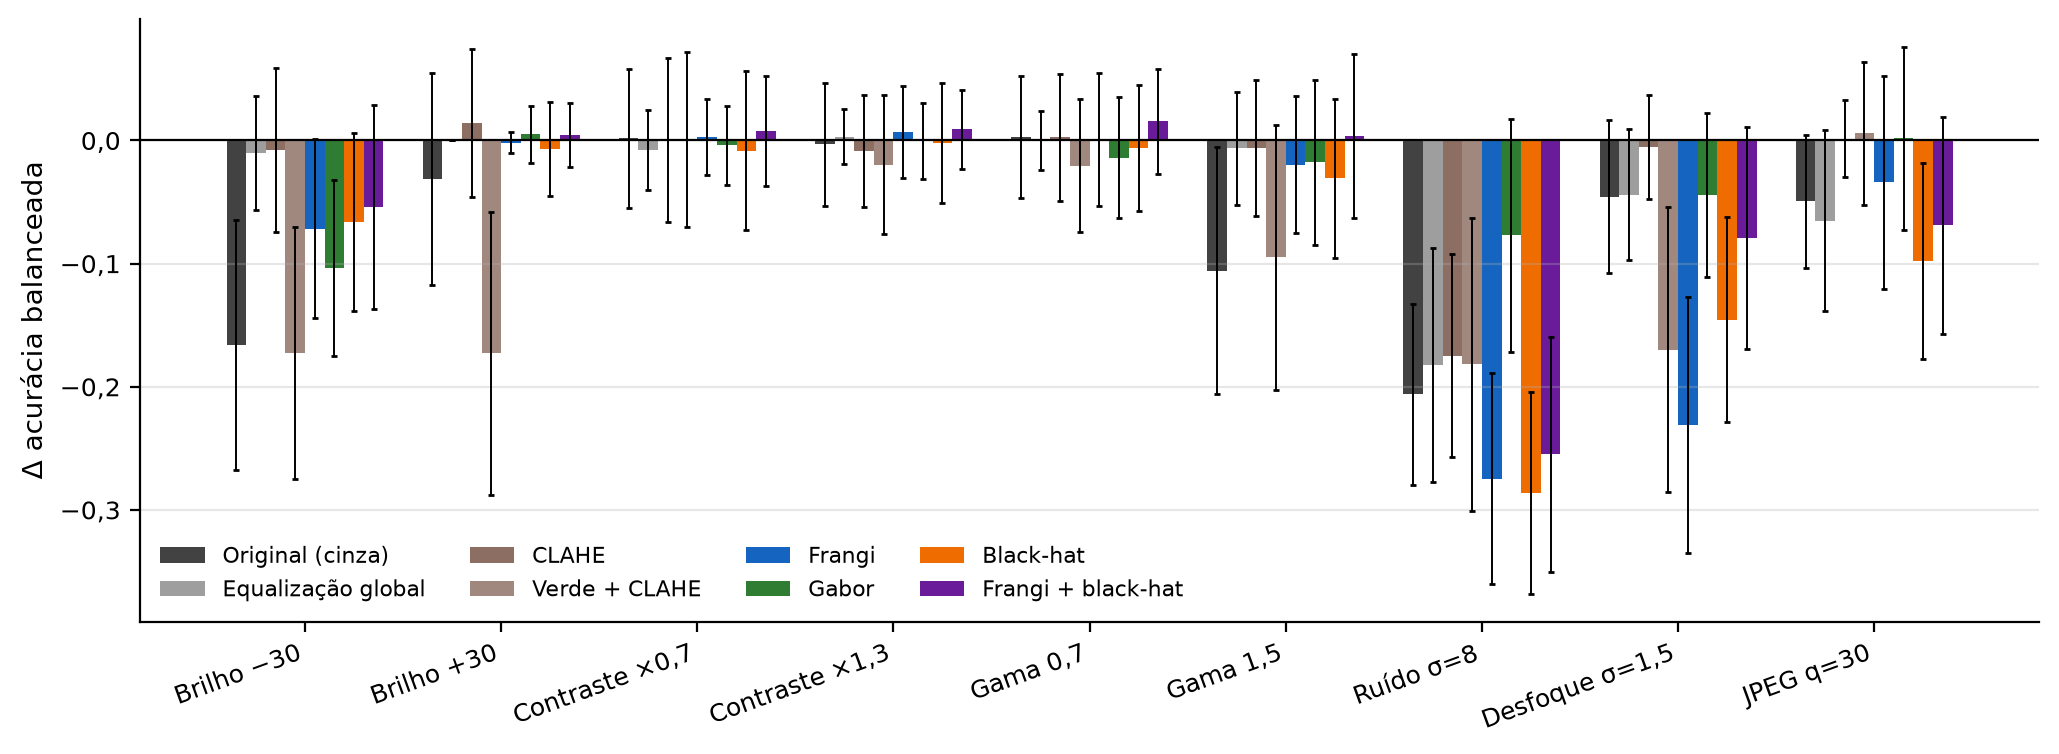
\includegraphics[width=\textwidth]{robustez_fotometrica.png}
  \par\medskip
  \footnotesize Fonte: elaborada pelo autor. Barras: média de 50
  \emph{folds}; hastes: intervalo de 95\% corrigido.
\end{figure}

\secao{A faixa normalizada não registra o tamanho da pupila}

A Figura~\ref{fig:invariancia} mostra a fotografia pública com a pupila
simulada em três tamanhos e as faixas normalizadas correspondentes, que são
visualmente indistinguíveis. No olho sintético com o modelo linear, o SSIM
entre a faixa de cada simulação e a de referência é de pelo menos
\val{b1-sint-lin-ssim} em toda a faixa de $\rho$ testada, como prevê a
Proposição~\ref{prop:invariancia}. No modelo não linear, o SSIM cai até
\val{b1-sint-nl-ssim} nos extremos: o traço indireto existe, mas é pequeno
diante da diferença entre íris diferentes (SSIM \val{b1-outras-ssim}). Na
fotografia real, com a pupila redetectada em cada imagem, o SSIM mínimo é
\val{b1-foto-ssim-min}; a redução decorre da perda de resolução radial quando
o anel afina e do erro residual da detecção. Ao mesmo tempo, $\rho$ medido
automaticamente acompanha o valor simulado, com erro absoluto médio de
\val{b1-sint-mae} no olho sintético e \val{b1-foto-mae} na fotografia.

\begin{figure}[htbp]
  \centering
  \caption{Invariância da faixa normalizada ao tamanho da pupila}
  \label{fig:invariancia}
  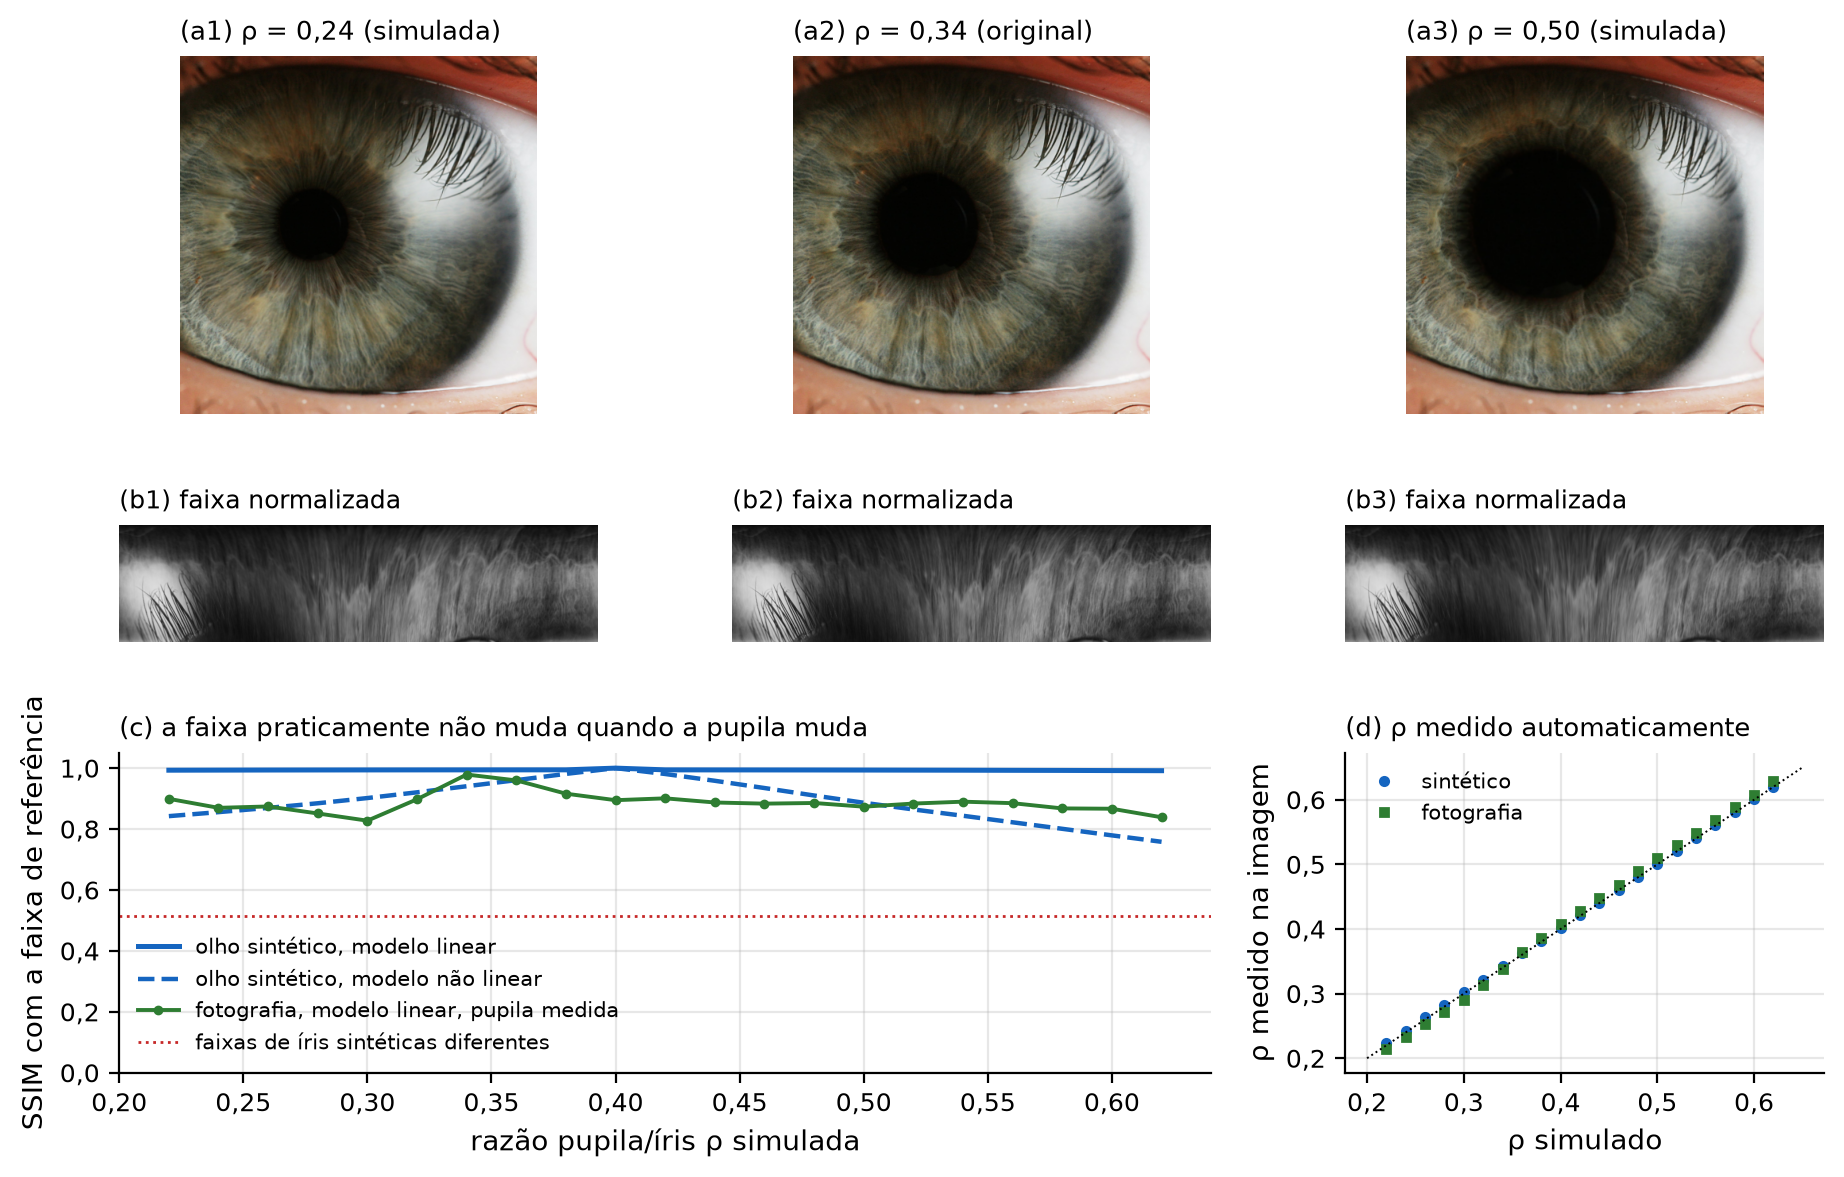
\includegraphics[width=\textwidth]{invariancia_rubber_sheet.png}
  \par\medskip
  \footnotesize Fonte: elaborada pelo autor. Painéis (a) e (b): fotografia de
  \citet{Novak2005} e simulações derivadas, sob CC BY-SA 2.5. Painéis (c) e
  (d): olho sintético e fotografia.
\end{figure}

\secao{Coorte sintética: faixa, geometria e fusão}

A Figura~\ref{fig:sinteticos} ilustra os olhos sintéticos e as faixas
normalizadas, que não mostram o tamanho da pupila. A
Tabela~\ref{tab:fatorial} e a Figura~\ref{fig:fatorial} trazem o
experimento $2\times2$. Sem efeito, todos os modelos ficam próximos de 0,5
(de \val{b2-nulo-oraculo} a \val{b2-nulo-faixa}), como esperado. Com o efeito
só na geometria, o pipeline restrito à faixa
fica em AUC \val{b2-geometria-faixa}, enquanto a geometria medida na
fotografia alcança \val{b2-geometria-geometria}, ao lado do oráculo
(\val{b2-geometria-oraculo}) e do limite teórico (\val{b2-teo}). Com o efeito
só na textura, os papéis se invertem: a faixa alcança
\val{b2-textura-faixa} e a geometria fica em \val{b2-textura-geometria}. Com
os dois efeitos, a fusão por empilhamento (\val{b2-ambos-fusao}) supera a
faixa (\val{b2-ambos-faixa}) e a geometria (\val{b2-ambos-geometria})
isoladas; nos cenários com um único efeito, a fusão acompanha o melhor
componente.

\begin{figure}[htb]
  \centering
  \caption{Olhos sintéticos com detecção automática e faixas normalizadas}
  \label{fig:sinteticos}
  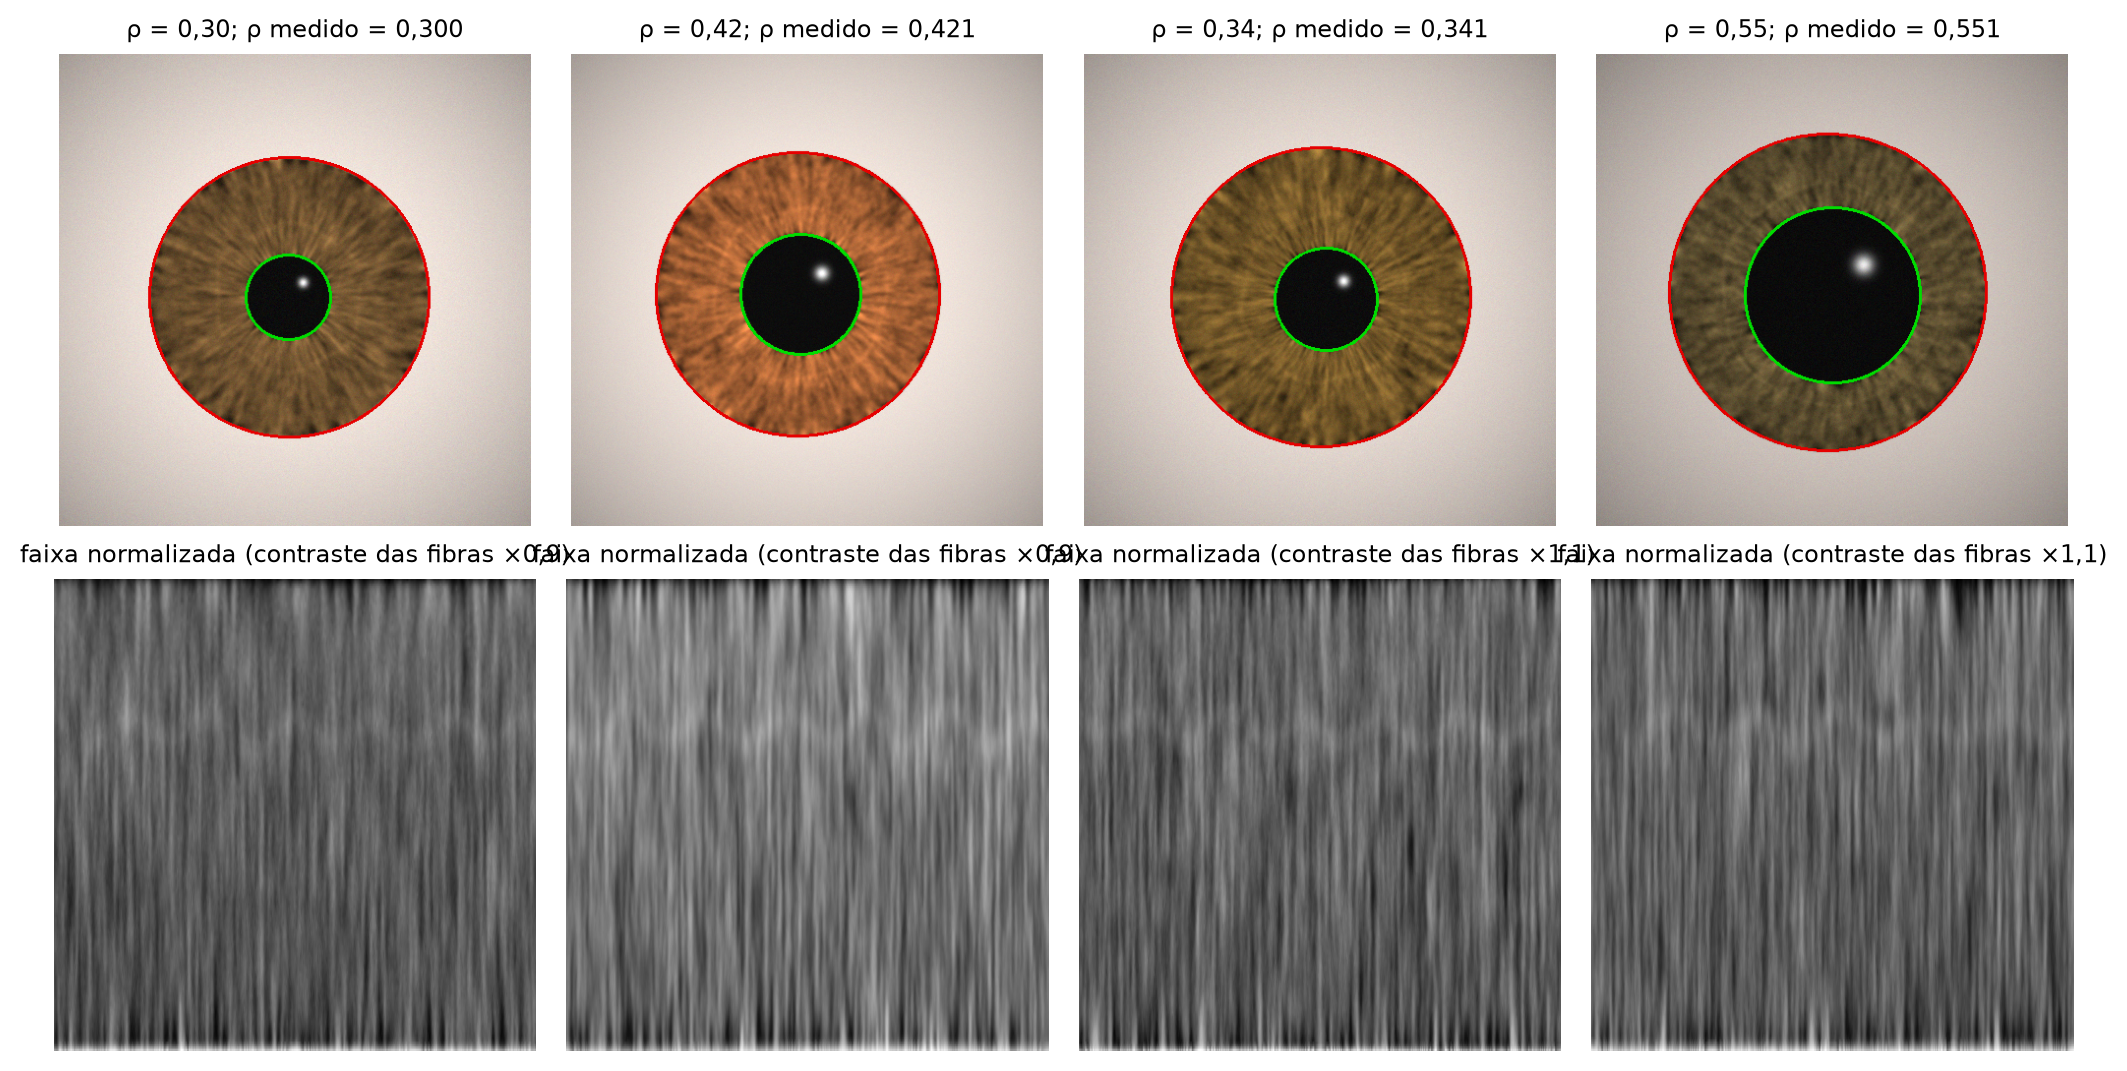
\includegraphics[width=\textwidth]{olhos_sinteticos.png}
  \par\medskip
  \footnotesize Fonte: elaborada pelo autor. Círculos: pupila (verde) e
  limbo (vermelho) detectados automaticamente.
\end{figure}

\begin{table}[htb]
  \centering
  \caption{AUC média (IC 95\% corrigido) na coorte sintética $2\times2$}
  \label{tab:fatorial}
  \footnotesize
  \resizebox{\textwidth}{!}{% Gerado por experiments/pgc3_pupil_geometry.py (não editar à mão).
\begin{tabular}{lcccc}
\toprule
Cenário & Faixa (IC) & Geometria medida & Fusão & Oráculo \\
\midrule
Sem sinal & 0,551 [0,49; 0,61] & 0,461 [0,38; 0,55] & 0,526 [0,45; 0,61] & 0,457 [0,37; 0,54] \\
Sinal só na geometria & 0,548 [0,47; 0,63] & 0,742 [0,65; 0,83] & 0,735 [0,65; 0,82] & 0,743 [0,65; 0,83] \\
Sinal só na textura & 0,870 [0,82; 0,92] & 0,529 [0,41; 0,64] & 0,870 [0,82; 0,92] & 0,531 [0,41; 0,65] \\
Sinal na geometria e na textura & 0,825 [0,78; 0,87] & 0,755 [0,68; 0,83] & 0,866 [0,82; 0,91] & 0,754 [0,68; 0,83] \\
\bottomrule
\end{tabular}
}
  \par\medskip
  \footnotesize Fonte: elaborada pelo autor. Validação cruzada estratificada
  $5\times5$ com \val{b2-n} olhos por classe em cada cenário.
\end{table}

\begin{figure}[htb]
  \centering
  \caption{AUC dos quatro modelos nos quatro cenários da coorte sintética}
  \label{fig:fatorial}
  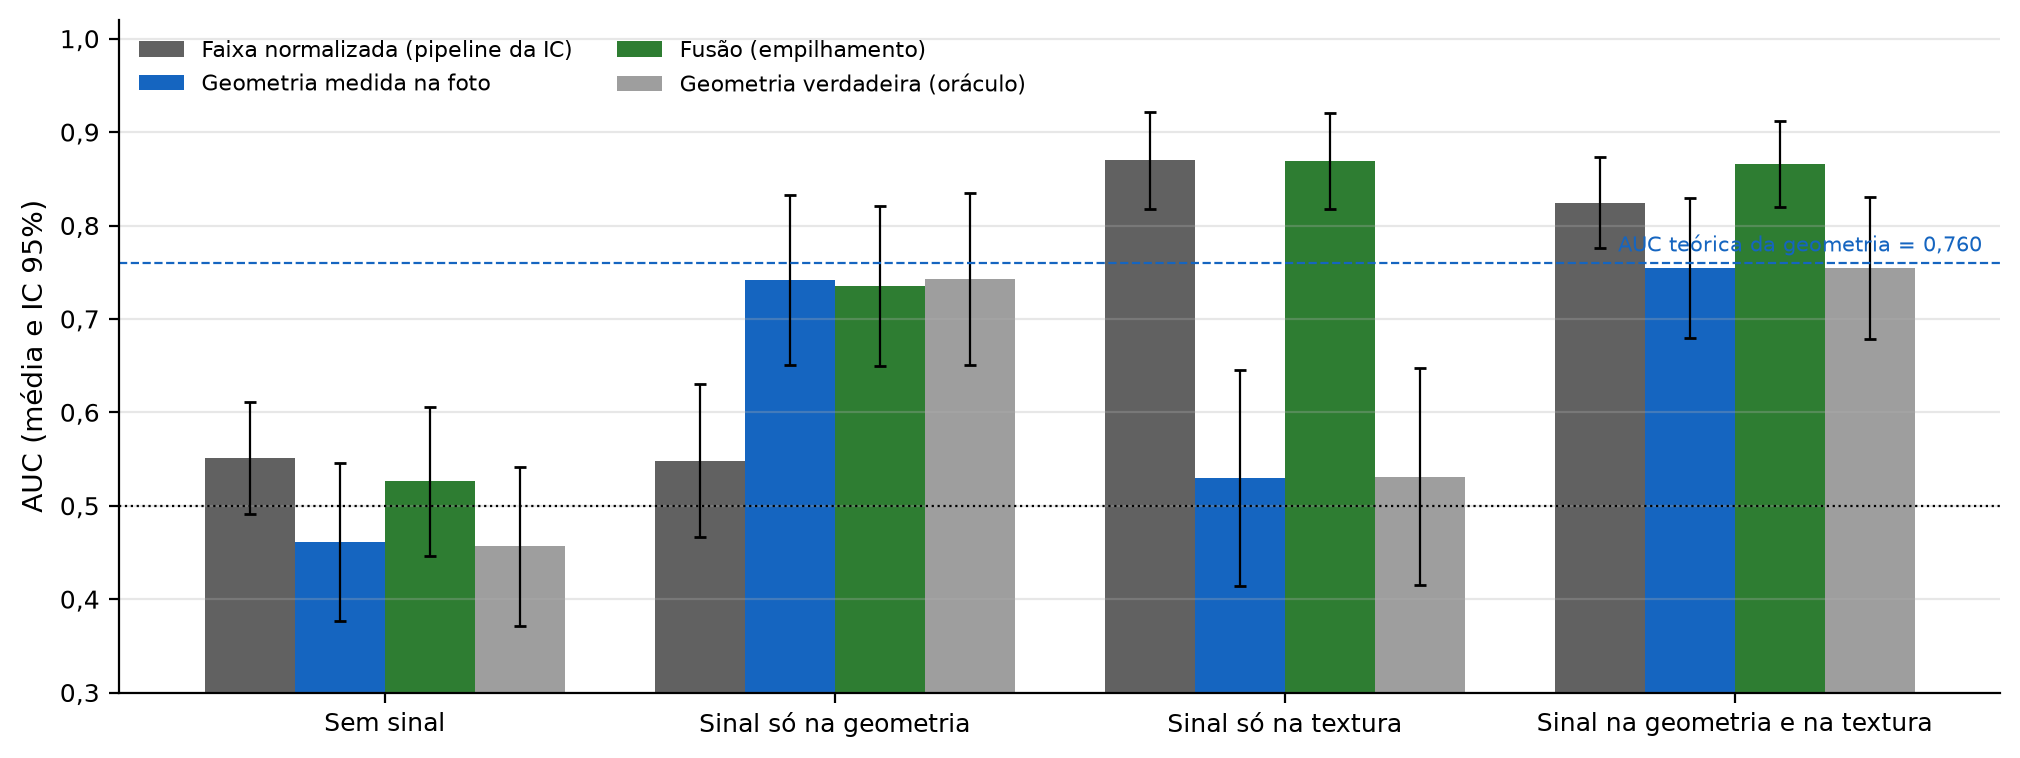
\includegraphics[width=\textwidth]{fatorial_pupila.png}
  \par\medskip
  \footnotesize Fonte: elaborada pelo autor.
\end{figure}

\secao{Medição automática de $\rho$}

A Tabela~\ref{tab:medicao} e a Figura~\ref{fig:medicao} comparam os
detectores. O segmentador por contornos ativos do pipeline da IC errou $\rho$
em mais de 0,03 em \val{b3-ic-falhas} dos \val{b3-ic-n} olhos testados, quase
sempre por superestimar a pupila, com tempo médio de \val{b3-ic-tempo}\,s por
imagem. O detector por limiar e Hough errou em mais de 0,03 em
\val{b3-demo-falhas} de \val{b3-demo-n} olhos (erro absoluto médio
\val{b3-demo-mae}), e seus erros se concentram nas pupilas pequenas. O motivo
está no limiar: quando a pupila ocupa menos de 3\% da imagem, o que nestas
imagens corresponde a $\rho$ abaixo de cerca de 0,33, o percentil 3 cai
dentro da íris, e a região escura limiarizada se estende além da pupila. Por
construção, esse detector também não encontra o limbo quando
$\rho>0{,}625$, porque sua busca por Hough começa em 1,6 vez o raio da
pupila. O detector desta etapa errou em \val{b3-starburst-falhas} de
\val{b3-starburst-n} olhos, com erro absoluto médio de \val{b3-starburst-mae},
viés de \val{b3-starburst-vies} e correlação de \val{b3-starburst-r} com o
valor verdadeiro.

\begin{table}[htb]
  \centering
  \caption{Erro na medição automática de $\rho$ na coorte sintética}
  \label{tab:medicao}
  \footnotesize
  \resizebox{\textwidth}{!}{% Gerado por experiments/pgc3_pupil_geometry.py (não editar à mão).
\begin{tabular}{lccc}
\toprule
Medida & Contornos ativos (IC)$^{*}$ & Limiar + Hough & \textit{Starburst} + refinamento \\
\midrule
Erro absoluto médio de $\rho$ & 0,279 & 0,0152 & 0,0012 \\
Erro absoluto mediano & -- & 0,0055 & 0,0012 \\
Percentil 95 do erro absoluto & -- & 0,0470 & 0,0022 \\
Maior erro absoluto & -- & 0,451 & 0,0034 \\
Viés (medido $-$ verdadeiro) & -- & 0,0145 & 0,0012 \\
Olhos com erro $>0{,}03$ & 11 de 12 & 81 de 800 & 0 de 800 \\
Correlação com $\rho$ verdadeiro & -- & 0,743 & 1,0000 \\
Tempo médio por imagem (s) & 7,5 & -- & 0,3 \\
\bottomrule
\end{tabular}
}
  \par\medskip
  \footnotesize Fonte: elaborada pelo autor. $^{*}$Subconjunto de
  \val{b3-ic-n} olhos, por causa do custo do segmentador.
\end{table}

\begin{figure}[htb]
  \centering
  \caption{$\rho$ medido contra $\rho$ verdadeiro para os três detectores}
  \label{fig:medicao}
  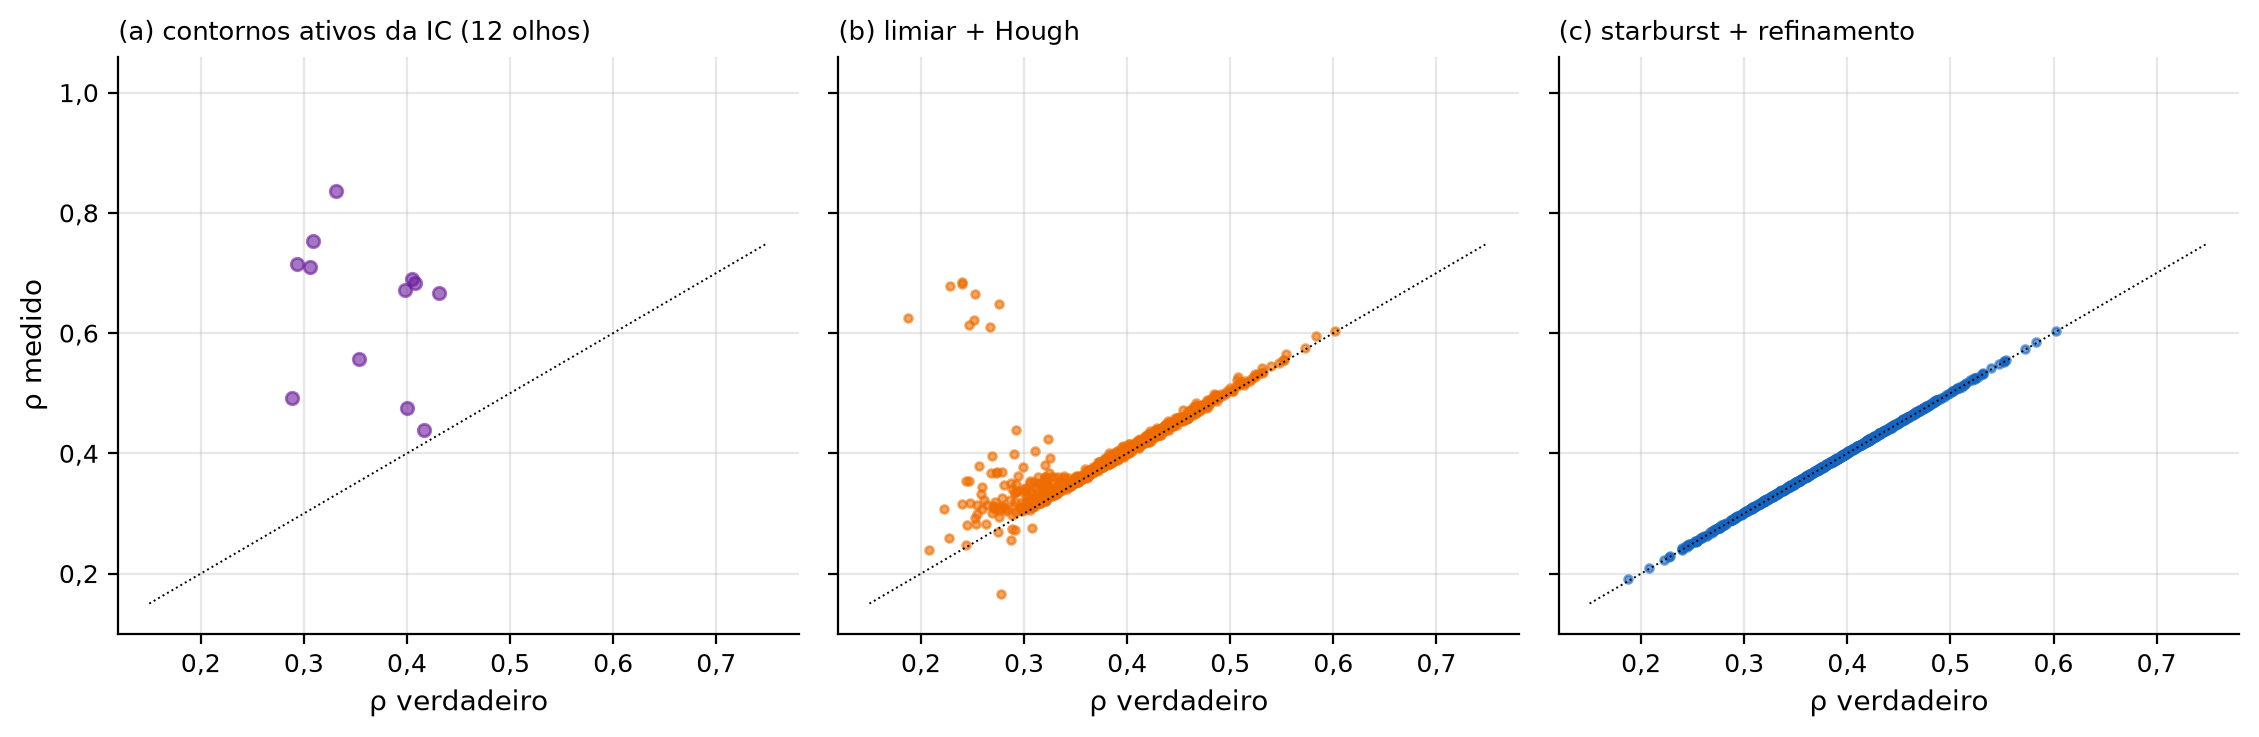
\includegraphics[width=\textwidth]{medicao_rho.png}
  \par\medskip
  \footnotesize Fonte: elaborada pelo autor.
\end{figure}

% ============================================================================
\chapter{Discussão}
\label{cap:discussao}

\secao{Pergunta 1: as imagens filtradas podem entrar diretamente no pipeline?}

Do ponto de vista técnico, sim: os realces entram no pipeline como qualquer
outra transformação, sem nenhum descritor novo, e classificam acima do acaso.
A pergunta de fundo, porém, era se essa entrada traria resultados
interessantes sobre a vascularização, e nesta base a resposta é negativa. O
ganho de cerca de 5 a 7 pontos percentuais observado com pixels no leiaute
principal não resistiu a três controles independentes: não se repetiu no
segundo leiaute; foi explicado em grande parte pelo espelhamento das faixas,
que prejudica a imagem original e quase não afeta os realces; e desapareceu
quando apenas o estroma foi usado, concentrando-se nas bordas pupilar e
límbica. A Hipótese~\ref{hip:realce} se confirma no mecanismo (os realces
removem os padrões de baixa frequência e deixam o pipeline menos sensível à
orientação das faixas), mas não na consequência esperada (uma separação
melhor das classes pela estrutura do estroma).

Dois achados reforçam essa leitura. Os descritores de textura da imagem
original são os mais altos e os mais estáveis nos dois leiautes, mas incluem o
histograma de intensidades, e oito estatísticas globais de cor bastam para AB
de \val{ctl-abmax-cor}: parte do sinal desta base está em propriedades globais
que podem refletir a aquisição das duas classes, e não a íris
\citep*{Zech2018,Geirhos2020}. Além disso, as bordas que concentram o sinal
dos realces são as regiões mais sensíveis à segmentação, à nitidez e à
iluminação. Elas também podem conter alterações do limbo associadas à idade,
que a base não permite controlar porque não registra a idade dos
participantes.

Quanto à alternativa dos descritores manuais, os 13 descritores calculados
sobre a resposta de Frangi alcançaram \val{ctl-abmax-manual} no melhor
classificador, sem superar a imagem filtrada nem a textura da original, e
incluem o terço externo da faixa, sujeito ao mesmo efeito de borda. Criar
descritores manuais de vascularização sobre esta base, portanto, não
resolveria o problema, que está na origem do sinal e não na forma de
representá-lo.

A robustez segue o mesmo padrão: as representações equalizadas e o Gabor são
as mais estáveis, enquanto Frangi e \bh{} perdem desempenho sob ruído e
desfoque. Na prática, a imagem filtrada é uma entrada viável, com desempenho
equivalente ao da imagem original e menor sensibilidade à orientação das
faixas, e o Gabor é o realce mais estável. Uma avaliação da vascularização
que mereça esse nome exige máscaras que excluam as bordas pupilar e límbica,
os controles de atalho usados aqui e dados com identificação por pessoa e
rótulos verificados.

\secao{Pergunta 2: a pupila precisa de descritores manuais?}

Precisa de descritores explícitos, mas não de trabalho manual. A
Proposição~\ref{prop:invariancia} e o experimento B1 mostram que a faixa
normalizada, que é o que o pipeline usa depois da segmentação, praticamente
não muda quando a pupila muda; o experimento B2 mostra que um efeito
puramente geométrico é invisível para o pipeline restrito à faixa e
recuperável quando $\rho$ entra como descritor, e que a fusão aproveita as
duas fontes quando ambas carregam sinal. A Hipótese~\ref{hip:geometria} se
confirma. Esses descritores ($\rho$, $\tau$ e $\epsilon$) são calculados
automaticamente a partir da própria fotografia, na etapa de segmentação;
nenhuma medida manual é necessária. Em resumo, o pipeline precisa da
fotografia do olho inteiro, e não apenas da faixa normalizada, e de um
caminho próprio para a geometria, implementado pela fusão por empilhamento.
O mesmo comportamento apareceu na execução do pipeline completo pela linha de
comando, com fotografias sintéticas.

Três observações completam a resposta. Primeiro, como $\tau=1-\rho$, o
diâmetro relativo da pupila e a espessura relativa do anel são uma única
variável; só a calibração em milímetros, ou uma medida de AS-OCT para a
espessura anatômica, acrescentaria informação nova. Segundo, a qualidade da
segmentação é decisiva: o segmentador por contornos ativos do pipeline da IC
não mediu $\rho$ corretamente em \val{b3-ic-falhas} dos \val{b3-ic-n} olhos
testados, e o detector desta etapa foi necessário. Terceiro, a base legada
não permite testar a pergunta com dados reais, porque contém apenas faixas
normalizadas, das quais a Proposição~\ref{prop:invariancia} mostra que $\rho$
não pode ser recuperado.

\secao{Limitações}

\begin{alineas}
  \item a base legada não tem identificadores de pessoa; olhos de uma mesma
  pessoa podem ter caído em \emph{folds} diferentes, o que tende a inflar
  todas as métricas, embora não favoreça uma representação em particular;
  \item a classe positiva é diabetes informado, sem verificação clínica nem
  confirmação do subtipo DM2, e o artigo associado à base foi retratado; os
  números são exploratórios e não estimam desempenho clínico;
  \item a segmentação original das faixas é desconhecida; as diferenças
  concentradas nas bordas podem refletir essa segmentação ou a aquisição, e
  não há como separá-las sem as fotografias originais;
  \item o leiaute principal mistura faixas espelhadas e não espelhadas, o que
  prejudica representações que dependem da posição angular;
  \item com \val{aud-unicas} imagens, os intervalos de confiança são largos, e
  as melhores combinações de cada representação (Apêndice~\ref{ap:tabelas})
  resultam de uma seleção otimista entre 15 alternativas;
  \item a coorte sintética demonstra o mecanismo, mas não estima o tamanho
  real do efeito pupilar no DM2, que depende da iluminação e do protocolo de
  aquisição; o tamanho do efeito de textura foi escolhido para equilibrar o
  desenho;
  \item os realces respondem a cílios, pálpebras e reflexos, que ainda não
  têm máscaras próprias.
\end{alineas}

% ============================================================================
\chapter{Conclusão e próximos passos}
\label{cap:conclusao}

As duas perguntas desta etapa têm respostas objetivas. Para a
vascularização, as imagens filtradas podem entrar diretamente no pipeline da
IC, sem descritores manuais, e classificam tão bem quanto a imagem original,
com a vantagem de serem menos sensíveis à orientação das faixas. Nesta base,
porém, o desempenho não pode ser atribuído à vascularização: o ganho aparente
dos realces não se repetiu no segundo leiaute, foi explicado em grande parte
pelo espelhamento das faixas e se concentrou nas bordas pupilar e límbica, e
não no estroma. Pelos mesmos motivos, descritores manuais de vascularização
não trariam ganho sobre esta base. Para a pupila, a faixa normalizada descarta
o tamanho da pupila, então a geometria precisa entrar como descritor
explícito; esse descritor é extraído automaticamente da fotografia, e o
pipeline já faz essa extração e a fusão. Os resultados negativos sobre a
vascularização são, eles próprios, uma contribuição: mostram que métricas
altas nesta base podem surgir de bordas, de orientação e de cor, e fornecem o
conjunto de controles que qualquer resultado futuro precisa atravessar.

Os próximos passos propostos para o PGC III são:
\begin{alineas}
  \item obter um conjunto com fotografias completas (não apenas faixas),
  identificadores de pessoa, diagnóstico de DM2 verificado, idade e protocolo
  de iluminação registrados, condição para testar a geometria pupilar em
  dados reais, separar olhos da mesma pessoa na validação cruzada e controlar
  o efeito da idade;
  \item aplicar máscaras que excluam as bordas pupilar e límbica, os cílios,
  as pálpebras e os reflexos antes do realce, e avaliar a vascularização
  apenas no estroma;
  \item manter, em qualquer novo conjunto, os controles introduzidos aqui:
  ablação do pré-processamento, atalho de cor, teste de permutação,
  replicação, recorte radial e correção para comparações múltiplas;
  \item dar preferência ao Gabor entre os realces, pelo equilíbrio entre
  desempenho e robustez, e padronizar a aquisição (foco, compressão e
  iluminação);
  \item calibrar $\rho$ em milímetros pelo diâmetro da íris e registrar a
  iluminação, para aproximar o diâmetro pupilar dos estudos clínicos;
  \item retomar os descritores manuais de vascularização apenas se, em dados
  adequados e restritos ao estroma, a imagem filtrada mostrar sinal que
  justifique uma descrição mais específica.
\end{alineas}
